\documentclass[11pt,a4paper]{ivoa}
\input ivoatex/tthdefs

\lstloadlanguages{sh,make,[latex]tex}
\lstset{flexiblecolumns=true,numberstyle=\small,showstringspaces=False,
  identifierstyle=\texttt,defaultdialect=[latex]tex,language=tex}

\usepackage{todonotes}
\usepackage{float}
\usepackage{adjustbox}
\usepackage{lscape}
\usepackage{makecell}
\usepackage{amsmath, amsthm, amssymb, amsfonts}

\usepackage[english]{babel}
\usepackage[font=footnotesize,labelfont=bf]{caption}
\usepackage{titlesec}

\usepackage[utf8]{inputenc}
\usepackage{float}
\usepackage[titletoc]{appendix}
\usepackage{listings}
% define colors for syntax XML 
% include listing settings 
\usepackage{listings}
\usepackage{color}
 
\definecolor{dkgreen}{rgb}{0,0.6,0}
\definecolor{OliveGreen}{rgb}{0.1,0.6,0.1}
\definecolor{gray}{rgb}{0.5,0.5,0.5}
\definecolor{mauve}{rgb}{0.58,0,0.82}
\definecolor{gray}{rgb}{0.4,0.4,0.4}
\definecolor{darkblue}{rgb}{0.0,0.0,0.6}
\definecolor{lightblue}{rgb}{0.0,0.0,0.9}
\definecolor{cyan}{rgb}{0.0,0.6,0.6}
\definecolor{darkred}{rgb}{0.6,0.0,0.0}


\lstset{
  basicstyle=\ttfamily\footnotesize,
  columns=fullflexible,
  showstringspaces=false,
  numbers=left,                   % where to put the line-numbers
  numberstyle=\tiny\color{gray},  % the style that is used for the line-numbers
  stepnumber=1,
  numbersep=5pt,                  % how far the line-numbers are from the code
  backgroundcolor=\color{white},      % choose the background color. You must add \usepackage{color}
  showspaces=false,               % show spaces adding particular underscores
  showstringspaces=false,         % underline spaces within strings
  showtabs=false,                 % show tabs within strings adding particular underscores
  frame=none,                   % adds a frame around the code
  rulecolor=\color{black},        % if not set, the frame-color may be changed on line-breaks within not-black text (e.g. commens (green here))
  tabsize=2,                      % sets default tabsize to 2 spaces
  captionpos=b,                   % sets the caption-position to bottom
  breaklines=true,                % sets automatic line breaking
  breakatwhitespace=false,        % sets if automatic breaks should only happen at whitespace
  title=\lstname,                   % show the filename of files included with \lstinputlisting;
                                  % also try caption instead of title  
  commentstyle=\color{gray}\upshape
}


\lstdefinelanguage{XML}
{
  morestring=[s][\color{mauve}]{"}{"},
  morestring=[s][\color{black}]{>}{<},
  morecomment=[s]{<?}{?>},
  morecomment=[s][\color{dkgreen}]{<!--}{-->},
  stringstyle=\color{black},
  identifierstyle=\color{lightblue},
  keywordstyle=\color{red},
  morekeywords={xmlns,xsi,noNamespaceSchemaLocation,type,id,source,target,version,tool,roleRef}
  }


% end define colors 



\usepackage{booktabs,xcolor}
\definecolor{texcolor}{rgb}{0.4,0.1,0.1}
\definecolor{lightgray}{gray}{0.9}

\lstset{flexiblecolumns=true,basicstyle=\ttfamily}

\iftth
  \newcommand{\BibTeX}{BibTeX}
\fi

\newcommand{\angstrom}{\mbox{\normalfont\AA}}

\title{IVOA Photometry Data Model}

\ivoagroup{Data Model Working Group}

\author{Jesús Salgado}
\author{Mireille Louys}
\author{Laurent Michel}
\author{Carlos Rodrigo}
\author{Pedro Osuna}
\author{Mark Allen}
\author{Jonathan McDowell}
\author{Deborah Baines}
\author{Jesús Maíz Apellániz}
\author{Evanthia Hatziminaoglou}
\author{Sebastien \mbox{Derriere}}
\author{Gerard Lemson}


\editor{Jesús Salgado}
\editor{Mireille Louys}


\begin{document}

\begin{abstract}
The Photometry Data Model (\textbf{PhotDM}) standard describes photometry 
filters, photometric systems, magnitude systems, zero points and its 
interrelation with the other IVOA data models through a simple data model. 
Particular attention is given necessarily to optical photometry where 
specifications of magnitude systems and photometric zero points are required 
to convert photometric measurements into physical flux density units.
\end{abstract}

\section*{Acknowledgments}
We acknowledge the EuroVO Science Advisory Committee for the review of the 
initial versions of the document and to the developers who have contributed 
to the data model reference implementations.
\pagebreak

\section*{Link to IVOA Architecture}
The figure below shows where IVOA Photometry Data Model fits within the 
IVOA architecture:


%%%%%%%%%%%%%%%%%%%% Figure/Image No: 1 starts here %%%%%%%%%%%%%%%%%%%%

\begin{figure}[H] 
\centering

% As of ivoatex 1.2, the architecture diagram is generated by ivoatex in
% SVG; copy ivoatex/archdiag-full.xml to archdiag.xml and throw out
% all lines not relevant to your standard.
% Notes don't generally need this.  If you don't copy archdiag.xml,
% you must remove archdiag.svg from FIGURES in the Makefile.

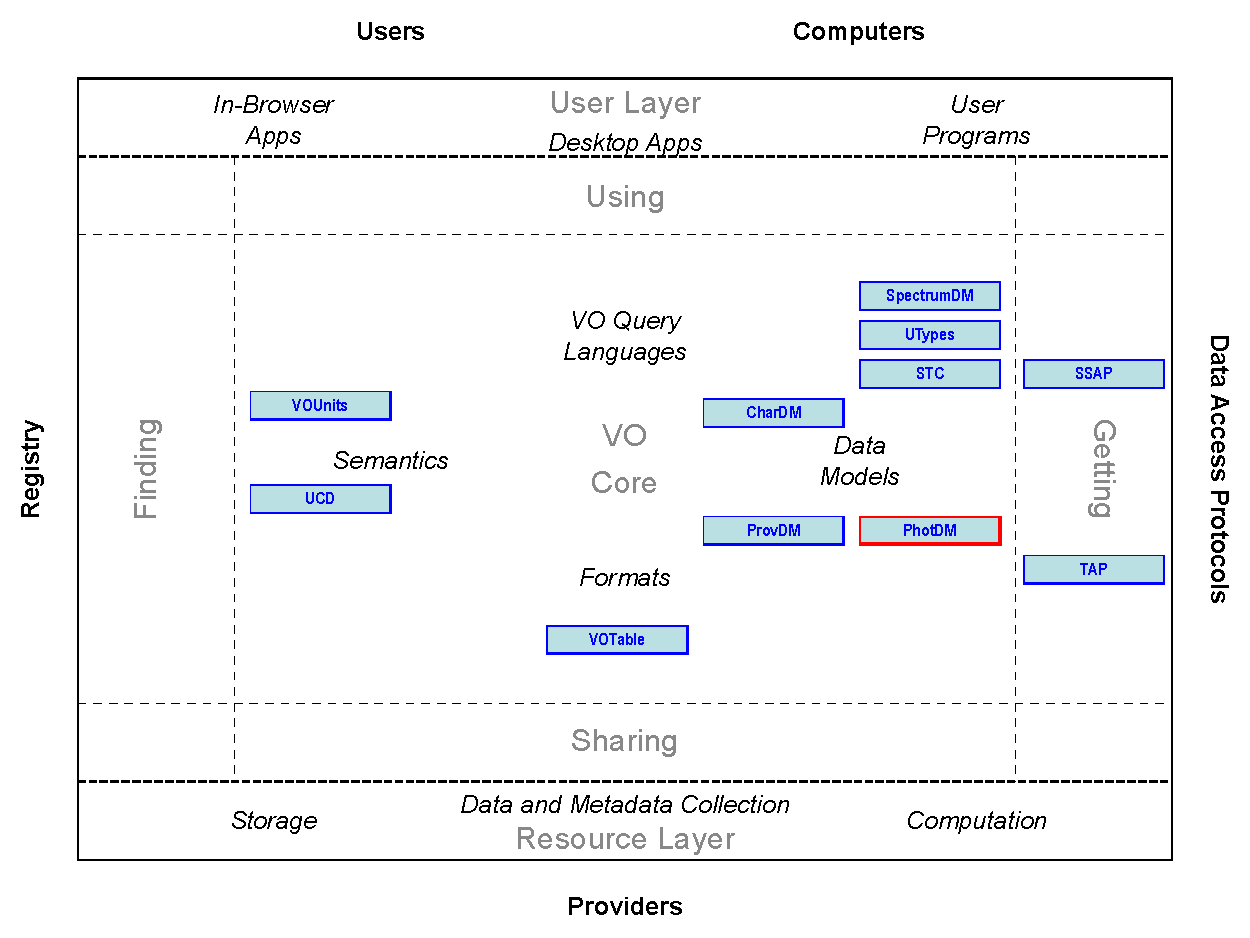
\includegraphics[width=0.9\textwidth]{role_diagram.pdf}
\caption{PhotDM can be used to enhance and abstract SSAP and TAP access, in particular 
to help on the automatic translation of magnitudes to fluxes and to add provenance 
metadata to these magnitudes. Also it can be used to generate SEDs using the SpectralDM.
PhotDM makes use of utypes from different IVOA data models, including CharDM and UCDs and
also express quantities in line with the VOUnits definition.
PhotDM also adds serialization examples in VOTable.
}
\label{fig:archdiag}
\end{figure}

\section*{Changes from Version 1.0} \label{changesTable}

%%%%%%%%%%%%%%%%%%%% change log starts here %%%%%%%%%%%%%%%%%%%%

\begin{table}[H]
 			\centering
\begin{tabular}{p{3.in}p{1in}p{0.8in}}
\hline
%row no:1
\multicolumn{1}{|p{3.75in}}{\textbf{Change}} &
\multicolumn{1}{|p{0.72in}}{\textbf{Section}} &
\multicolumn{1}{|p{0.9in}|}{\textbf{Date}} \\
\hline

%row no:2
\multicolumn{1}{|p{3.75in}}{First PhotDM 1.1 Latex version} &
\multicolumn{1}{|p{0.72in}}{All} &
\multicolumn{1}{|p{0.9in}|}{{\fontsize{10pt}{12.0pt}\selectfont 
2021/10/07}} \\
\hline

%row no:3
\multicolumn{1}{|p{3.75in}}{Use the Modelio class diagram 
figure} &
\multicolumn{1}{|p{0.72in}}{\ref{datamodel}} &
\multicolumn{1}{|p{0.9in}|}{{\fontsize{10pt}{12.0pt}\selectfont 
2021/10/25}} \\
\hline

%row no:4
\multicolumn{1}{|p{3.75in}}{Data model summary updates and 
correction of UCD tags} &
\multicolumn{1}{|p{0.72in}}{All} &
\multicolumn{1}{|p{0.9in}|}{{\fontsize{10pt}{12.0pt}\selectfont 
2021/12/21}} \\
\hline

%row no:5
\multicolumn{1}{|p{3.75in}}{Add changes table} &
\multicolumn{1}{|p{0.72in}}{\ref{datamodel}} &
\multicolumn{1}{|p{0.9in}|}{{\fontsize{10pt}{12.0pt}\selectfont 
2022/02/02}} \\
\hline

%row no:5
\multicolumn{1}{|p{3.75in}}{Add mapping example} &
\multicolumn{1}{|p{0.72in}}{\ref{appendixmapping}} &
\multicolumn{1}{|p{0.9in}|}{{\fontsize{10pt}{12.0pt}\selectfont 
2022/03/01}} \\
\hline

%row no:6
\multicolumn{1}{|p{3.75in}}{v1.1 Proposed Recommendation} &
\multicolumn{1}{|p{0.72in}}{All} &
\multicolumn{1}{|p{0.9in}|}{{\fontsize{10pt}{12.0pt}\selectfont 
2022/03/01}} \\

\hline
\end{tabular}
\end{table}
\pagebreak

\section{Introduction}
A key role of the VO is to help astronomers find data and to 
combine that data in a scientifically meaningful way. A Spectral 
Energy Distribution (SED) is an example of combining data whereby 
flux density measurements of an astrophysical source at different 
spectral energy coordinates (wavelengths/frequencies/energy)
(\citep{doi:10.1146/annurev.astro.41.082801.100251}, 
\citep{longo}, \citep{connell}, \citep{brujine}) are plotted as a 
graph of flux density versus a spectral energy coordinate. SEDs that 
cover a wide range of the electromagnetic spectrum are particularly 
useful for identifying the underlying physical processes operating 
in the astrophysical source, and the use of SEDs is becoming more 
prevalent as astronomy takes an increasingly multi-wavelength 
approach. To combine individual flux density measurements and their 
spectral energy coordinates into an SED, these phometric measurements 
must be described in sufficient detail to allow for the conversion to 
compatible flux density and spectral energy units,  taking into 
account the nature of the spectral energy bandpass of the measurements, 
as well as the apertures and other details of  the measurements. 
This document outlines a photometry data model to describe photometric 
measurements in a standard way.

The photometry data model aims to describe the essential elements 
of flux density measurements made within all spectral energy domains 
across the electromagnetic spectrum. In some domains this is 
relatively straight forward, such as in radio astronomy where 
measurements are commonly expressed in flux density units, and 
where data are readily combined into SEDs. The data model fields 
required to describe such a radio flux density measurement includes 
a specification of the bandpass, the units of the measurement and 
the associated uncertainties. Optical photometry measurements are 
however commonly expressed in magnitudes, and a greater level of 
description of the magnitude systems and bandpasses are required 
to support the conversion of these measurements into flux densities 
that could be combined into an SED. As such, much of this document 
is necessarily devoted to defining the data model fields required 
to describe optical photometry measurements.

Astronomical flux density measurements will often require a 
greater level of description than provided by this simple model. 
The level of accuracy required depends strongly on the scientific 
use of the data. A study of broadband SEDs of active galaxies may 
tolerate 20$\%$  uncertainties in the flux density measurements, 
and it is usually sufficient in these cases to use average values 
for the spectral energy coordinates of the bandpasses. Fitting to 
stellar models or science that employs photometric measurements to 
derive photometric redshifts requires a much greater level of accuracy. 
To manage the different levels of description we take the overall 
approach that the photometry data model should include the most 
generic elements required to describe photometric measurements, 
and that the photometry data model is intended to be used in 
coordination with the IVOA Spectrum Data model and the IVOA 
Characterization Data Model.

The scientific use case that has guided the choice of the level 
of description of the metadata fields in the Photometry Data Model 
is the use of the large collections of photometric data that are 
published in catalogues (e.g. Vizier, \url{http://vizier.u-strasbg.fr/}) 
in SEDs. The Photometry Data Model provides the metadata fields for 
describing the photometry measurements in catalogues, so that those 
data could then be added to, or compared with an SED.

The intended practical use of the Photometry Data Model is that the 
metadata fields defined here will be included in the metadata of 
catalogues, or of photometry data stored as a pseudo-spectrum. These 
data would then be made accessible using Simple Spectral Access Protocol 
(SSAP) or Table Access Protocol (TAP) services so that the photometric 
measurements can be used and combined in scientific software tools.

The proposed model is based on the description of the photometry 
filters, and the description of how\ the\ units of the measurement 
are related to flux density. The photometry filter description may 
be as simple as specifying a central spectral energy coordinate and 
a bandpass width. The more detailed description of optical bandpasses 
is supported by allowing for specification of filter transmission 
curves, and the   photometric zero points necessary for the conversion 
of magnitudes to flux densities.

Information on the properties of filters is not always easily available, 
and is sometimes only specified in manuals or in the literature and often 
not in digital form. To aid the use of filters information, in particular 
as part of the Photometry Data Model metadata fields, we propose a 
mechanism for referencing external filter information. Such a 
\textit{Filter Profile Service} would expose this information so software 
client applications could discover it. This document proposes a 
standardization of a protocol to be used by Filter Profile Services.


The following sections of this document summarize some key points 
about astronomical photometry (Section 2). The detailed metadata 
structure of the data model is presented in Section 3. Section 4 
describes use cases in which the model description could be used in 
making photometry data available through VO protocols, and, very briefly, 
how scientific tools could use this information.


PhotDM is related to other IVOA Data models (Spectrum DM, Characterization DM, 
Observation and Provenance DM),  and is intended to provide photometry 
metadata for data that would be accessed via the IVOA Data Access Protocols 
such as SSAP (Simple Spectra Access Protocol) or TAP (Table Access Protocol).

As with most of the VO Data Models, PhotDM makes use of STC, Utypes, Units 
and UCDs. PhotDM will be serializable with a VOTable.

\section{Astronomical Photometry}
Astronomical photometry refers to measuring the brightness, flux or 
intensity of an astrophysical object. Consider an astronomical source 
with a flux density at the observer $F(x)$, where $x$ is a spectral coordinate 
(wavelength, frequency or energy).  The photometry measurement will be related 
to $<F>$ a flux weighted integral of this flux density over an observed band 
with a relative spectral response $T(x)$. The flux weighted integral in its most 
simple form is defined as


\begin{equation} \label{eq:1}
\langle F\rangle = \int F(x)T(x)dx 
\end{equation}

Calibration of photometric measurements is in general done by comparison to a 
reference spectrum that has a known effective flux density $f_0$ at a specific 
spectral band.


For this reference spectrum, the flux weighted integral is defined as:

\begin{equation} \label{eq:2}
\langle F_R \rangle= \int F_R (x)T(x)dx 
\end{equation}


so that the effective flux density of the source can be evaluated as:

\begin{equation} \label{eq:3}
f = f_0 ( \frac{\langle F\rangle }{\langle F_R \rangle } ) 
\end{equation}

This represents the most simple and easy to use flux measurement. Flux 
measurements expressed in physical flux density units can be easily combined 
into SEDs. Many flux measurements published in catalogues of radio sources 
for example are simple flux densities of this form.
\par

In optical photometry measurements are often expressed as magnitudes and it 
is necessary to define the magnitude system being used, and the zero point 
fluxes of the reference spectrum.
\par

Pogson magnitudes are defined as:

\begin{equation} \label{eq:4}
m = -2.5\log_{10} (\langle F\rangle ) 
\end{equation}

which when compared to a reference spectrum $F_R$ leads to:

\begin{equation} \label{eq:5}
m = m_R -2.5 \log_{10} \left(\langle F\rangle /\langle F_R \rangle \right) 
\end{equation}

As explained above, this is equivalent to:

\begin{equation} \label{eq:6}
m = m_R - 2.5 \log_{R} (f/f_0 )
\end{equation}


so that

\begin{equation} \label{eq:7}
f = f_0 10^{-0.4(m - m_{R})}
\end{equation}


Using this expression a measurement in magnitudes can be converted to a 
flux density, given the zero point flux of the reference spectrum.  The 
magnitude of reference $m_{R}$ and the zero point $f_0$ will be defined 
in the document. $m_{R}$ is most often chosen to be zero (or one for 
linear photometric systems) in most of the photometric systems although, 
usually, continuous recalibration of the photometric system usually 
produces a deviation of this value.
\par

There are a number of magnitude systems that are defined by the reference 
spectrum. The three most commonly used magnitude systems are the Vega 
magnitude, $AB_{\nu }$ magnitude and $ST_{\lambda }$ magnitude systems. 
The Vega magnitude system uses the spectrum of Vega (Alpha Lyrae) as the 
reference spectrum $F_R (x)$. The $AB_{\nu }$ magnitude system uses 
reference spectrum defined by a constant flux density per unit frequency 
($F_{\nu }$) and the
$ST_{\lambda }$ magnitude system uses a reference spectrum of a constant 
flux density per unit wavelength ($F_{\lambda }$). The values of $F_{\nu }$ 
and $F_{\lambda }$ that respectively define the zero points
$m_{AB,\nu } =0$ and
$m_{ST,\lambda } =0$ have been chosen to be the mean flux density of 
Vega in the Johnson V band.

\begin{equation} \label{eq:7}
m_{AB,\nu } = 0
\end{equation}

\begin{equation} \label{eq:8}
f_\nu = 3.63\times 10^{-20}\,erg\,cm^{-2}\,s^{-1}\,Hz^{-1}
\end{equation}

\begin{equation} \label{eq:9}
m_{ST,\lambda } = 0
\end{equation}

\begin{equation} \label{eq:10}
f_\lambda = 3.63\times 10^{-9}\,erg\,cm^{-2}\,s^{-1}\,\angstrom^{-1}
\end{equation}


A convenient graphical representation of these systems is shown in 
Figure 3.1 of the Synphot manual:

\url{http://www.stsci.edu/resources/software_hardware/stsdas/synphot/SynphotManual.pdf}.
\par

For a photometric system that uses Vega magnitudes, the zero point 
flux for each filter is the average flux density of Vega over that 
bandpass $f_{Vega}$. Some typical values of $f_{Vega}$ are tabulated in 
(\citep{2001eaa..book.....M}) for the Johnson photometric system. Although 
the agreed Vega spectrum has changed historically, the commonly referred to 
spectrum of Vega in digital form described in (\citep{2004AJ....127.3508B}) 
is available as file at alpha\_lyr\_stis\_002.fits at:\par
\url{http://www.stsci.edu/instruments/observatory/cdbs/calspec}
\par

In the AB system, the flux density (in units of $erg\, cm^{_2}\, s^{-1}\, Hz^{-1}$) 
corresponding to a given magnitude is simply obtained via:

\begin{equation} \label{eq:11}
f_{\nu} = 10^{-0.4(m_{AB}+48.6)}
\end{equation}

And, in the same way, in the ST system, the flux density (in units of $erg\, 
cm^{_2}\, s^{-1}\, \angstrom^{-1}$) corresponding to a given magnitude is:

\begin{equation} \label{eq:12}
f_{\lambda} = 10^{-0.4(m_{ST}+21.1)}
\end{equation}

Another magnitude system is the Asinh magnitude system in which magnitudes 
are defined as
\begin{equation} \label{eq:13}
m = \frac{2.5}{ln(10)} \left[ sinh^{-1}(\frac{f}{2bf_0}) +ln(b) \right]
\end{equation}


where b is known as the softening parameter. Details of the Asinh magnitude 
system and the softening parameters are described in 
\url{http://www.sdss.org/DR7/algorithms/photometry.html}
\par

\section{Photometry Data Model} \label{datamodel}
The model shown in Figure 1, organizes the structure and detailed metadata 
fields of the Photometry Data Model in a logical manner, and shows the 
relationship to other IVOA data models. The metadata fields for each class 
specify the essential elements required to describe a photometric measurement.
\par

The main class in this diagram is Photometry Filter. This class contains 
all the attributes necessary to describe a filter from the data discovery 
point of view.
\par

A Photometric System is a grouping of individual Photometry Filters. This may 
represent a particular set of filters that are related in some way.
\par

A magnitude system is characterised for a certain reference spectrum that 
will produce a certain zero point for a certain photometry filter. This 
reference spectrum could be an ideal one (as in STmag and ABmag systems), a 
Vega-like spectrum (as in Vegamag systems) (please notice that different Vega 
spectrum versions have been historically used) or any other. In many cases, 
the reference spectrum has been calculated as an average of spectra from several 
astronomical objects. This would be characterised by a set of Source instances.
\par

A zero point would then be a flux value that can be considered as zero 
magnitude, so its value will allow conversions from fluxes to magnitudes 
and the other way around. It has associated a photometry filter and it also 
depends on the magnitude system (reference spectrum) used to calculate this 
magnitude.
\par

There are different types of zero points (Pogson, asinh, linear etc) that will 
essentially differ in the way that getFluxFromMagnitude and getMagnitudeFromFlux 
operators are implemented plus extra information that could be needed to do 
these conversions.
\par

An intermediate class, PhotCal, can be understood as a certain photometry 
filter instance, i.e., a certain photometry filter using a certain magnitude 
system and linked to a certain zero point class. PhotCal is the class node 
where data model describing spectral data interacts. It binds the filter and 
zeropoint information to the Flux Axis calibration. It can be understood as the 
calibration configuration used , bringing together a specific photometry filter 
instance with magnitude system and zeropoint. It leverages the handling of 
photometric data through IVOA protocols e.g. SSAP or TAP services.
\par

A Spectrum would have a Characterization Coordsys element that will have 
associated a certain PhotCal element in the case of photometry data. Using 
this information, magnitudes from different photometric systems could be 
compared between them or compared to spectroscopic data expressed in flux.
\par

%%%%%%%%%%%%%%%%%%%% Figure/Image No: 22 starts here %%%%%%%%%%%%%%%%%%%%
% -- MireilleLouys
% I would prefer to use the diagram I provided in Modelio,
% because it traces more details on the associations, and contains the 
% descriptions inserted in
% the generated VO-DML xml file
% the file for replacement will be 
% "./schema/PhotDMv1-1-overview diagram-2021-04-12.png"
% -- Mireille Louys
\begin{figure}[H]
%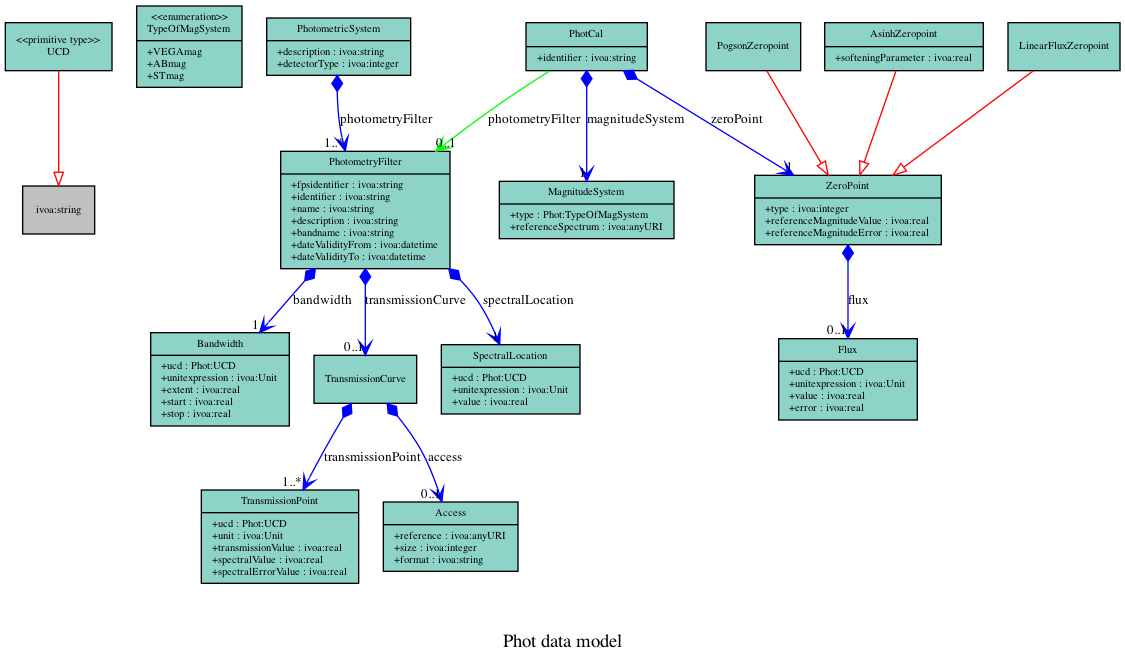
\includegraphics[angle=90,width=5.98in,height=7.19in]{./schema/PhotDMv1-1.png}
% update Mireille new diagram
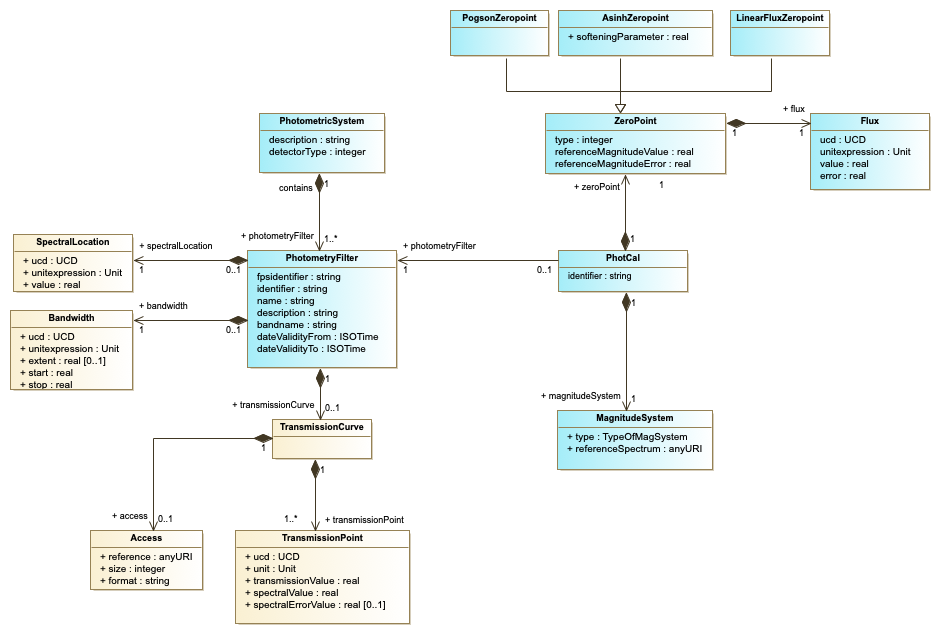
\includegraphics[angle=90,width=5.98in,height=7.19in]{./schema/PhotometryOverviewDiagram_jan22.png}
\caption{Class diagram of the Photometry Calibration Data Model: All 
classes are defined in VO/DML view at: 
\url{https://github.com/ivoa-std/PhotDM/photdm/schema/}}
\end{figure}


%%%%%%%%%%%%%%%%%%%% Figure/Image No: 22 Ends here %%%%%%%%%%%%%%%%%%%%



 %%%%%%%%%%%%  Starting New Page here %%%%%%%%%%%%%%

\newpage

 %%%%%%%%%%%%  Starting New Page here %%%%%%%%%%%%%%

\newpage
In order to fully describe values of the magnitudes inside photometry point 
instances, the class diagram makes use of physical quantity classes. These 
classes glue all the basic fields that compose a physical measurement: value, 
error, units, etc. However, within the present specification, we will describe 
individual attributes of the different quantities and as a consequence. All 
the utypes will be also generated from individual physical quantity 
attributes what will facilitate the use within IVOA Data Access Layer protocols.
\par

\subsection{PhotometricSystem Class}
This class briefly describes the photometric system that contains a set of 
photometry filters. Photometry filters can be contained in a certain 
photometric system as part of the same observatory/telescope or as part 
of a known system.
\par

\subsubsection{PhotometricSystem.description: String}
This String contains a human readable short-text representation of the 
photometric system. This will allow client applications to display 
textual information to final users.
\par

Examples:

%%%%%%%%%%%%%%%%%%%% Table No: 2 starts here %%%%%%%%%%%%%%%%%%%%

%row no:1
Sloan \par
Johnson
\bigskip

%%%%%%%%%%%%%%%%%%%% Table No: 2 ends here %%%%%%%%%%%%%%%%%%%%


\subsubsection{PhotometricSystem.detectorType: integer}
Detector type associated to this photometric system. Possible 
values are:


%%%%%%%%%%%%%%%%%%%% Table No: 3 starts here %%%%%%%%%%%%%%%%%%%%


\begin{table}[ht]
 			\centering
\begin{tabular}{p{2.42in}p{0.8in}p{1.55in}}
\hline
%row no:1
\multicolumn{1}{|p{2.42in}}{Type of detector} &
\multicolumn{1}{|p{0.8in}}{Value} &
\multicolumn{1}{|p{1.55in}|}{Examples} \\
\hline
%row no:2
\multicolumn{1}{|p{2.42in}}{Energy Counter} &
\multicolumn{1}{|p{0.8in}}{0 (default)} &
\multicolumn{1}{|p{1.55in}|}{Energy amplifiers devices} \\
\hline
%row no:3
\multicolumn{1}{|p{2.42in}}{Photon Counter} &
\multicolumn{1}{|p{0.8in}}{1} &
\multicolumn{1}{|p{1.55in}|}{CCDs or photomultipliers} \\
\hline
\end{tabular}
\caption{Detector Types}
 \end{table}


%%%%%%%%%%%%%%%%%%%% Table No: 3 ends here %%%%%%%%%%%%%%%%%%%%

This will be used in order to decide how to calculate the 
flux average in, e.g., the synthetic photometry calculations. 
At current state, this list is exhaustive. See photometry filter 
transmission curve description to understand how to use this field.
\par

\subsection{PhotometryFilter Class}
This is the main class that describes a photometry filter.
\par

\subsubsection{PhotometryFilter.identifier: String}
This field identifies, in a unique way, within a certain Photometry 
Filter Profile service, a filter. Although the main requirement of 
this data model field is to be unique within a Filter Profile Service, 
the suggested syntax would be:
\par

%%%%%%%%%%%%%%%%%%%% Table No: 4 starts here %%%%%%%%%%%%%%%%%%%%

%row no:1
Facility/Subcategory/Band[/Suffix]
\bigskip

%%%%%%%%%%%%%%%%%%%% Table No: 4 ends here %%%%%%%%%%%%%%%%%%%%

where \textit{Facility} is the telescope, observatory, space mission, 
etc that has this filter, \textit{Subcategory} is a meaningful 
classification of filters within a facility (usually instrument), 
\textit{Band} is the generic name used to describe the wavelength 
band used by this filter and \textit{Suffix} is optional metadata added 
to the unique identifier string to ensure uniqueness within a Filter 
Profile Service.
\par

Example:
\par
%%%%%%%%%%%%%%%%%%%% Table No: 5 starts here %%%%%%%%%%%%%%%%%%%%
SDSS/SDSS.G/G
\bigskip

%%%%%%%%%%%%%%%%%%%% Table No: 5 ends here %%%%%%%%%%%%%%%%%%%%

\subsubsection{PhotometryFilter.fpsIdentifier: String}
IVOA identifier of the filter profile service where this photometry 
filter is registered to be used in the discovery of all the relevant 
photometry filter properties.
\par

This identifier follows the IVOA syntax defined for IVOA 
identifiers (\citep{plante}) which gives a string built up as:
\par

%%%%%%%%%%%%%%%%%%%% Table No: 6 starts here %%%%%%%%%%%%%%%%%%%%
ivo://<ivoa authority id>/<resource key>
\bigskip



%%%%%%%%%%%%%%%%%%%% Table No: 6 ends here %%%%%%%%%%%%%%%%%%%%

Example:
\par

%%%%%%%%%%%%%%%%%%%% Table No: 7 starts here %%%%%%%%%%%%%%%%%%%%
ivo://svo/fps
\bigskip



%%%%%%%%%%%%%%%%%%%% Table No: 7 ends here %%%%%%%%%%%%%%%%%%%%

where svo is the authority id, fps is the resource key of the service.
\par

Whenever the definition of the FPS filter profile service is standarised,
the service url of the filter profile service could be obtained 
from the registry by requesting the associated information of this 
registry resource, e.g., once registered the service URL associated 
to this Filter Profile Service would be, e.g.:
\par

%%%%%%%%%%%%%%%%%%%% Table No: 8 starts here %%%%%%%%%%%%%%%%%%%%
http://svo.cab.inta-csic.es/theory/fps/
\bigskip

%%%%%%%%%%%%%%%%%%%% Table No: 8 ends here %%%%%%%%%%%%%%%%%%%%
At this stage, only one filter profile service exists so the service
URL would be the previously mentioned.

\subsubsection{PhotometryFilter.name: String}
This String contains a human readable representation of the filter 
name. This will allow client applications to display information 
to the final user.
\par

Example:
\par

%%%%%%%%%%%%%%%%%%%% Table No: 9 starts here %%%%%%%%%%%%%%%%%%%%
SDSS.G
\bigskip



%%%%%%%%%%%%%%%%%%%% Table No: 9 ends here %%%%%%%%%%%%%%%%%%%%

\subsubsection{PhotometryFilter.description: String}
This String contains a verbose human readable string description of the 
filter. This will allow client applications to display text information 
to the final user.
\par

\subsubsection{PhotometryFilter.bandName: String}
This String contains a standard representation of the spectral band 
associated to this filter (if any). This information is useful for human 
interpretation but it is discourage to use it for discovery purposes. The 
reason is that a filter is not always properly represented by a standard 
band so filters could be lost in a query response.
\par

Examples:
\par


%%%%%%%%%%%%%%%%%%%% Table No: 10 starts here %%%%%%%%%%%%%%%%%%%%
U \par B  \par V
\bigskip

%%%%%%%%%%%%%%%%%%%% Table No: 10 ends here %%%%%%%%%%%%%%%%%%%%

Where U,B,V corresponds to ultraviolet, blue and visible respectively.
\par

\subsubsection{PhotometryFilter Time Validity Range}
The following fields will be used to characterize the validity range of 
this specific photometry filter configuration. This is particularly useful 
for ground based telescopes where filter, electronics, etc could easily 
change generating versions of the same photometry filter.
\par

\paragraph{PhotometryFilter.dateValidityFrom: ISOTime}
Start time of the time coverage when this filter configuration is 
applicable. The value is specified as in DALI \citep{2017ivoa.spec.0517D} 
timestamps\par

%%%%%%%%%%%%%%%%%%%% Table No: 11 starts here %%%%%%%%%%%%%%%%%%%%
YYYY-MM-DD[T[hh[:mm[:ss[.s]]]]]
\bigskip


%%%%%%%%%%%%%%%%%%%% Table No: 11 ends here %%%%%%%%%%%%%%%%%%%%

\paragraph{PhotometryFilter.dateValidityTo: ISOTime}
End time of the time coverage when this filter configuration is 
applicable. The value is specified as in DALI \citep{2017ivoa.spec.0517D} 
timestamps\par


%%%%%%%%%%%%%%%%%%%% Table No: 12 starts here %%%%%%%%%%%%%%%%%%%%
YYYY-MM-DD[T[hh[:mm[:ss[.s]]]]]
\bigskip

%%%%%%%%%%%%%%%%%%%% Table No: 12 ends here %%%%%%%%%%%%%%%%%%%%

\subsubsection{PhotometryFilter.transmissionCurve}
Here we consider how wavelengths/frequencies are filtered in the whole 
acquisition chain for a calibrated observation stemming from a given 
data collection.
\par

This means that within the same data collection most observations will 
point to the same PhotometryFilter.transmissionCurve.
\par

The effective transmission curve may be represented as a 2-D graph that 
describes the transmission properties of the filter over a wavelength 
range defined by the filter bandpass.
\par

It is composed of a spectral coordinate in the x-axis and a scalar in 
the y-axis. This effective response curve encloses all the possible 
components that modifies the energy/photon collection, including detector, 
telescope and even atmosphere for transmission curves referenced in 
measurements. 
Most modern surveys try to reduce everything according to a given airmass 
(e.g. 1.3) and this is particularly important for ground-based filters 
with $\lambda < 4000 \angstrom $ or  $\lambda > 7000 \angstrom $.
\par

%%%%%%%%%%%%%%%%%%%% Figure/Image No: 3 starts here %%%%%%%%%%%%%%%%%%%%
\begin{figure}[H]
	\begin{center}
		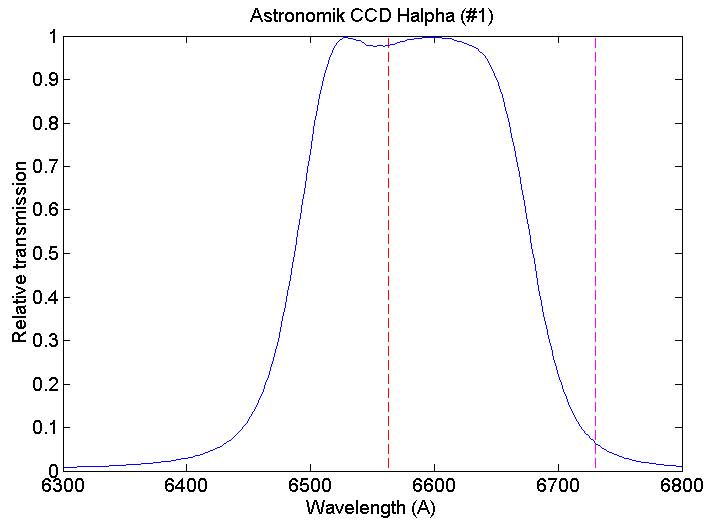
\includegraphics[width=4.24in,height=3.12in]{./media/image25.png}
		\caption{Transmission Curve example}
	\end{center}
\end{figure}

%%%%%%%%%%%%%%%%%%%% Figure/Image No: 3 Ends here %%%%%%%%%%%%%%%%%%%%

\par

This curve can be used, e.g. for the creation of synthetic photometry 
(\citep{1996BaltA...5..459S},\citep{2004A&A...422..205G}) from an observational 
or a theoretical spectrum by applying it to the spectrum in the filter band-pass. 
Taking as input a certain flux, the effective flux as seen using a certain 
filter would be, for energy counters (\citep{2007ASPC..364..227M}):

\begin{equation} \label{eq:14}
f(\lambda_{eff}) = \frac{\int T(\lambda)F(\lambda)d\lambda}{\int T(\lambda)d\lambda}
\end{equation}

And for photon counters (like CCDs or photomultipliers):

\begin{equation} \label{eq:15}
f(\lambda_{eff}) = \frac{\int T(\lambda)F(\lambda)\lambda d\lambda}{\int T(\lambda)\lambda d\lambda}
\end{equation}

Where $T(\lambda)$ is the transmission curve, $f(\lambda)$ is the flux of 
the spectrum. As the transmission curve is defined only in the filter 
band-pass, the limits of the integrals corresponds to the spectral range where 
the transmission curve is defined (stored as \textit{PhotometryFilter.bandwidth} 
in this data model)
\par

The transmission curve can be closely (although not fully) identified as an array 
of points as in a spectrum. There are various ways to provide this information 
either directly in an embedded table, or using a reference to a serialised table 
file.
\par

Spectral and transmission coordinates can be gathered directly as a table using 
TransmissionPoint utypes (see \ref{serializationfilter})\textit{.}.
\par

\subsubsection{PhotometryFilter.spectralLocation.value: double}
A spectral coordinate value that can be considered by the data provider as the 
most representative for this specific filter band-pass. The selection of this 
value should take into account the filter transmission curve profile and in 
general should be close to the wavelength mean value, defined 
(\citep{1982AJ.....87..670O}) as:
\par
\begin{equation} \label{eq:16}
\lambda_{mean} = \frac{\int T(\lambda)\lambda d\lambda}{\int T(\lambda)d\lambda}
\end{equation}

where $\lambda_{mean}$ is the spectral bounds mean value, $T(\lambda)$ is 
the transmission curve (see below), $\lambda$ is the wavelength. Please 
notice that, since the transmission curve will only be defined in a specific 
spectral range, the integrals will also be effectively defined in this 
spectral range.
\par

Another convenient definition of an effective wavelength is the 
$``$pivot wavelength$"$  defined as follows:

\begin{equation} \label{eq:17}
\lambda_{pivot} = \sqrt{\frac{\int T(\lambda)\lambda d\lambda}{\int T(\lambda)\frac{d\lambda}{\lambda}}}
\end{equation}

It can be proved that the pivot wavelength fulfills the following 
relation between the $f_\lambda$ and  $f_\nu $:

\begin{equation} \label{eq:18}
\langle f_\nu \rangle =\langle f_\lambda \rangle \lambda^2_{pivot}/c
\end{equation}

Other definitions for effective wavelengths commonly used in the literature 
are source dependent as, e.g., the isophotal wavelength:
\begin{equation} \label{eq:19}
\lambda_{mean} = \frac{\int \lambda F_\lambda(\lambda)T(\lambda)d\lambda}{\int F_\lambda(\lambda)T(\lambda)d\lambda}
\end{equation}

Or the photon distribution based effective wavelength:
\begin{equation} \label{eq:20}
\lambda_{mean} = \frac{\int \lambda^2 F_\lambda(\lambda)T(\lambda)d\lambda}{\int \lambda F_\lambda(\lambda)T(\lambda)d\lambda}
\end{equation}

but these source dependent definitions have two caveats:

\begin{itemize}
	\item{Real spectra do not necessarily satisfy the requirements of the mean value theorem, 
	which could produce multiple values for the wavelength.}

	\item{Calculation of these wavelengths implies the knowledge of $F_\lambda $ (usually 
	what you want to measure) and it does not look like an intrinsic property of the 
	photometry filter.}
\end{itemize}\par

\subsubsection{PhotometryFilter.transmissionCurve}
This data model field stores points of the curve in place in a simple table using spectrum 
data fields as shown above. See serialization example in \ref{serialization} section 
\ref{serializationfilter} \par

\paragraph{3.2.9.1 PhotometryFilter.transmissionCurve.access} \hspace{0pt} \\
If the transmission curve is hooked as an external file, we use the \textit{Access} class 
defined in the Observation CoreComponents data model (\citep{louys2011ivoa}) and inherited 
from the SSA specification (\citep{2012ivoatody}).
\par

\subparagraph{3.2.9.1.1 PhotometryFilter.transmissionCurve.access.reference} 
\hspace{0pt} \\
The access reference is a URI (typically a URL) which can be used to retrieve the 
specific dataset described in a row of the query table response. \par

\subparagraph{3.2.9.1.2 PhotometryFilter.transmissionCurve.access.format} \hspace{0pt} \\
The PhotometryFilter.transmissionCurve.access.format data model field tells the MIME 
type of the file pointed to and used to store the curve points. Values for this 
string can generally be:\par

%%%%%%%%%%%%%%%%%%%% Table No: 13 starts here %%%%%%%%%%%%%%%%%%%%
application/fits \par
application/x-votable+xml \par
text/csv \par
text/xml
\bigskip


%%%%%%%%%%%%%%%%%%%% Table No: 13 ends here %%%%%%%%%%%%%%%%%%%%

The file content will be a spectrum serialization with 
\textit{PhotometryFilter.transmissionCurve.spectrum.Dataset.DataModel }set to 
$``$Spectrum1.1$"$  for instance , and all necessary fields for the spectral and 
flux coordinates.
\par

\subparagraph{3.2.9.1.3 PhotometryFilter.transmissionCurve.access.size} 
\hspace{0pt} \\
Approximate estimated size of the dataset, specified in kilobytes. This would 
help the client estimate download times and storage requirements when generating 
execution plans. Only an approximate, order of magnitude value is required (a value 
rounded up to the nearest hundred kB would be sufficient).\par

\paragraph{3.2.9.2 PhotometryFilter.transmissionCurve.transmissionPoint} 
\hspace{0pt} \\
The transmission curve is a mathematical function that describes the transmission 
fraction of a certain filter in a defined spectral range. This function can be discretised 
as a set of transmission points and every point will be composed by two attributes:
\par

\begin{itemize}
	\item One spectral coordinate (wavelength, energy or frequency) value, of type 
	PhysicalQuantity, and utype:\par

\begin{center}
{\fontsize{10pt}{12.0pt}\selectfont 
\textbf{\textit{photDM:PhotometryFilter.transmissionCurve.
transmissionPoint.spectralValue}}\par}
\end{center}\par

	\item One transmission unitless value between 0 and 1 of type double and 
	utype:{\fontsize{11pt}{13.2pt}\selectfont \textit{ }\par}
\end{itemize}\par

\begin{center}
{\fontsize{10pt}{12.0pt}\selectfont \textbf{\textit{photDM:PhotometryFilter.transmissionCurve.
transmissionPoint.transmissionValu}e}\par}
\end{center}\par

\subparagraph{3.2.9.2.1
PhotometryFilter.transmissionCurve.transmissionPoint.
spectralValue.UCD: String} \hspace{0pt} \\
This data model field contains a Unified Content Description string (UCD) 
(\citep{2007ivoa.spec.0402M}) that specifies the nature of the spectral axis for this filter. 
This applies to the full spectral axis description of the filter.
\par

Example:
\par



%%%%%%%%%%%%%%%%%%%% Table No: 14 starts here %%%%%%%%%%%%%%%%%%%%
em.wl
\bigskip



%%%%%%%%%%%%%%%%%%%% Table No: 14 ends here %%%%%%%%%%%%%%%%%%%%

Where \textit{em.wl }indicates that the spectral coordinate is provided in wavelength.
\par

The Unit and UCD strings follow specific constraints defined in the IVOA standards and are 
implemented using type restrictions on strings.
\par

\subsubsection{PhotometryFilter.bandwidth: S\_Bounds}
A reference position along the spectral axis coverage of the referenced photometry filter.
\par

Although this will partially reuse the
\par

\begin{center}
Char.SpectralAxis.Coverage.Location.Bounds
\end{center}\par

concept of the Characterization Data Model, the basic elements of this object are described 
within the context of a photometry filter as follows.
\par

\paragraph{3.2.10.1
PhotometryFilter.bandwith.UCD: String} \hspace{0pt} \\
Unified Content Description (UCD) string that specifies the nature of the bandwidth object.
\par

\paragraph{3.2.10.2
PhotometryFilter.bandwith.unit: IVOA.Unit} \hspace{0pt} \\
Field that specifies the units of the bandwidth object.
\par

\paragraph{3.2.10.3
PhotometryFilter.bandwith.extent: double} \hspace{0pt} \\
For square filters (100$\%$  between the minimum and maximum wavelength and 0$\%$  otherwise), 
the bandwidth could be described as $\lambda_{max} - \lambda_{min}$.
\par

However, for real filters, the bandwidth is not very usable to describe the band-pass of the 
filter, but the effective width, that can be described as follow:
\begin{equation} \label{eq:21}
w = \frac{\int T(\lambda)d\lambda}{Max(T(\lambda))}
\end{equation}

where $w$ is the effective width, $T(\lambda)$ is the transmission curve (see below) 
and $Max(T(\lambda))$ the maximum value of the transmission curve. As in previous points, 
please notice that, since the transmission curve will be only defined in a specific spectral 
range, the integrals will also be defined in this spectral range.
\par

\paragraph{3.2.10.4
PhotometryFilter.bandwith.start: double } \hspace{0pt} \\
Also called in the rest of the document, this is a spectral value that better describes 
the reasonable minimum value of the spectral range of the filter band-pass. In general,
although this 
will not be imposed in order to allow a better description for different types of 
transmission curves, this quantity will be close to:
\begin{equation} \label{eq:22}
\lambda_{min} = \lambda_{mean} - \frac{w}{2}
\end{equation}

In practice, this could be taken as the minimum value of the filter transmission curve.
\par

\paragraph{3.2.10.5
PhotometryFilter.bandwith.stop: double} \hspace{0pt} \\
Also called $\lambda_{max}$ in the rest of the document, this is a spectral value that 
better describes the reasonable maximum value of the spectral range of the filter band-pass. 
In general, 
although this will not be imposed in order to allow a better description for different 
types of transmission curves, this quantity will be close to:
\begin{equation} \label{eq:23}
\lambda_{min} = \lambda_{mean} + \frac{w}{2}
\end{equation}

In practice, this could be taken as the maximum value of the filter transmission 
curve.\par

\subsection{PhotCal Class}
PhotDM is a class to describe the use of a photometry filter by using a certain magnitude system 
configuration. It has associated a certain zero point object.
\par

\subsubsection{PhotCal.identifier: String}
This field identifies, in a unique way, within a certain Photometry Filter Profile 
service, a zero point assigned to a filter and a certain photometric system type. 
Although the main requirement of the uniqueIdentifier is to be unique within a Filter 
Profile Service, the suggested syntax would be:
\par

%%%%%%%%%%%%%%%%%%%% Table No: 15 starts here %%%%%%%%%%%%%%%%%%%%
Facility/Subcategory/Band/Photometric System Type[/Suffix]
\bigskip


%%%%%%%%%%%%%%%%%%%% Table No: 15 ends here %%%%%%%%%%%%%%%%%%%%
where \textit{Facility} is the telescope, observatory, space mission, etc that 
has this filter, \textit{Subcategory} is a meaningful classification of filters 
within a facility (usually instrument), \textit{Band} is the generic name used to 
describe the wavelength band used by this filter \textit{Photometric System Type} 
makes reference to the type of system as per classification within this document 
and \textit{Suffix} is optional metadata added to the unique identifier string to 
ensure uniqueness within a Filter Profile Service.
\par

Please notice the suggested syntax of PhotCal unique identifier syntax corresponds 
with the Photometry Filter unique identifier concatenated with the photometric 
system type.
\par

Example:
\par



%%%%%%%%%%%%%%%%%%%% Table No: 16 starts here %%%%%%%%%%%%%%%%%%%%
SDSS/SDSS.G/G/AB
\bigskip


%%%%%%%%%%%%%%%%%%%% Table No: 16 ends here %%%%%%%%%%%%%%%%%%%%


\subsubsection{PhotCal.zeroPoint: ZeroPoint}
Zero point object associated to this PhotCal instance.
\par

\subsubsection{PhotCal.magnitudeSystem: MagnitudeSystem}
Magnitude system object associated to this phot cal instance.
\par

\subsection{ZeroPoint Class}
This class is used to characterize a zero point flux obtained during the 
calibration of a certain photometry filter on a certain photometric system 
configuration. This object includes references to the relevant Photometric 
System and Photometry Filter objects.
\par

\subsubsection{ZeroPoint.flux.value: double}
Flux of an astronomical object that produces a magnitude of reference 
(usually set as zero) for this particular filter and photometric system. 
This quantity is necessary to convert to flux a certain magnitude.
\par

For Pogson magnitudes (see section 3.2.5) it will be used in the following way:
\par
\begin{equation} \label{eq:24}
f = f_0 10^{-(m-m_R )/2.5}
\end{equation}

See ZeroPoint.type description for other definitions.
\par

The flux could be expressed as $f_{\lambda}$ or $f_{\nu}$, leaving the 
characterization of the type of flux to the units in which this quantity 
is expressed.
\par

\subsubsection{ZeroPoint.referenceMagnitude.value: double}
Most of the time, the zero point flux is defined for a magnitude=0 value. 
However, to give room to other cases, another reference magnitude value can 
be given instead of zero. The use of this reference magnitude is described in 
the different getMagnitudeFromFlux() and getFluxFromMagnitude() zero point 
extension operations.
\par

Please notice that, by default, reference magnitude will be zero unless 
specified otherwise.
\par

The reference magnitude is a dimensionless variable. It is modeled using a 
PhysicalQuantityDouble object type.
\par

\subsubsection{ZeroPoint.referenceMagnitude.error: double}
Total error estimated of the reference magnitude whenever applicable. Reference 
Magnitude error is a dimensionless variable.\par

\subsubsection{ZeroPoint.type: enum}
Usual definition of magnitudes, also called Pogson magnitudes, can be improved 
for faint sources by replacing the usual logarithm with an inverse hyperbolic 
sine function. These kinds of magnitudes are called $``$asinh magnitudes$"$  
or $``$luptitudes$"$  (\citep{2004A&A...422..205G})\par

%%%%%%%%%%%%%%%%%%%% Table No: 17 starts here %%%%%%%%%%%%%%%%%%%%


\begin{table}[ht]
 			\centering
\begin{tabular}{p{2.42in}p{0.8in}p{1.55in}}
\hline
%row no:1
\multicolumn{1}{|p{2.42in}}{Zero point type} &
\multicolumn{1}{|p{0.8in}}{Value} &
\multicolumn{1}{|p{1.55in}|}{Description} \\
\hline
%row no:2
\multicolumn{1}{|p{2.42in}}{Pogson} &
\multicolumn{1}{|p{0.8in}}{0 (default)} &
\multicolumn{1}{|p{1.55in}|}{Usual definition} \\
\hline
%row no:3
\multicolumn{1}{|p{2.42in}}{Asinh} &
\multicolumn{1}{|p{0.8in}}{1} &
\multicolumn{1}{|p{1.55in}|}{Used for faint sources, replacing the usual 
logarithm with an inverse hyperbolic sine function.} \\
\hline
%row no:4
\multicolumn{1}{|p{2.42in}}{LinearFlux} &
\multicolumn{1}{|p{0.8in}}{2} &
\multicolumn{1}{|p{1.55in}|}{Linear (not logarithmic) magnitudes used in 
Radio, Far Infrared, X-Ray spectral } \\
\hline
\end{tabular}
\caption{Types of Zero Points}
 \end{table}


%%%%%%%%%%%%%%%%%%%% Table No: 17 ends here %%%%%%%%%%%%%%%%%%%%

The main difference between the three types of zero points is the 
conversion formulae to be used when translating magnitudes into flux and 
reverse.\par

In the ZeroPoint class we define two conversion functions; 
getMagnitudeFromFlux() and getFluxFromMagnitude() defined as:\par

\begin{itemize}
	\item getMagnitudeFromFlux()\par

\begin{itemize}
	\item{Input Parameters: Flux given in units defined in the 
	ZeroPoint.unit data model field.\par}

	\item{Output Result: Corresponding magnitude in double.\par}


\vspace{\baselineskip}

\end{itemize}
	\item  getFluxFromMagnitude()\par

\begin{itemize}
	\item{Input Parameters: Magnitude in double\par}

	\item{Output Result: Corresponding flux given in units defined in 
	the ZeroPoint.unit data model field.}
\end{itemize}
\end{itemize}
\par


\subsection{PogsonZeroPoint Class}
Extension of ZeroPoint to accommodate standard logarithm magnitudes. It 
has no supplementary attributes but specific conversion functions.
\par

\subsubsection{PogsonZeroPoint.getFluxFromMagnitude()}
Operator to convert from a flux to a magnitude for Pogson magnitudes. For 
Pogson magnitudes, the usual definition should be used:
\par
\begin{equation} \label{eq:25}
f = f_0 10^{-(m-m_R)/2.5}
\end{equation}

Where $f$ is the associated flux, $f_0$ is the flux of reference, $m_0$ is 
the magnitude of reference (by default equals to zero) and $m$ is the 
observed magnitude.
\par

\subsubsection{PogsonZeroPoint.getMagnitudeFromFlux()}
Operator to convert from a flux to a magnitude for Pogson magnitudes. 
For Pogson magnitudes, the usual definition should be used:
\begin{equation} \label{eq:26}
m = m_R - 2.5\log(\frac{f}{f_0 })
\end{equation}

Where $f$ is the associated flux, $f_0$ is the flux of reference, 
$m_R$ is the magnitude of reference (by default equals to zero) and 
$m$ is the observed magnitude.
\par

\subsection{AsinhZeroPoint Class}
Extension of ZeroPoint  to describe asinh magnitudes, a.k.a. luptitudes.
\par

\subsubsection{AsinhZeroPoint.softeningParameter: double}
Parameter used to correct the calculation of magnitudes for faint 
sources. Usually called b. See (\citep{1999AJ....118.1406L}) for 
a formal explanation.
\par

Example:
\par

%%%%%%%%%%%%%%%%%%%% Table No: 18 starts here %%%%%%%%%%%%%%%%%%%%

\begin{table}[ht]
\centering
    \begin{tabular}{m{2.7cm}m{8cm}}
	\hline %inserts double horizontal lines
Band & Softening Parameters (b coefficients) \\
\hline
 $U$ & $1.4 \times 10^{10}$ \\
 $G$ & $0.9 \times 10^{10}$ \\
 $R$ & $1.2 \times 10^{10}$ \\
 $I$ & $1.8 \times 10^{10}$ \\
 $Z$ & $7.4 \times 10^{10}$ \\
\hline
\end{tabular}
\caption{Values used for SDSS DR5 asinh magnitudes}

\end{table}


%%%%%%%%%%%%%%%%%%%% Table No: 18 ends here %%%%%%%%%%%%%%%%%%%%

\subsubsection{AsinhZeroPoint.getFluxFromMagnitude()}
For asinh magnitudes, the operator to be used is:\par
\begin{equation} \label{eq:27}
f = f_0 10^{-(m-m_R )/2.5} \left[ 1-b^2 10^{2(m-m_R )/2.5}\right]
\end{equation}

Where $f$ is the flux of the observed source, $f_0$ is the zero 
point flux value, $m$ is the magnitude assigned to this source, 
$m_0$ is the reference magnitude (default value to zero unless 
specified otherwise) and a new parameter appears, $b$, called the 
softening parameter which is referenced in this data model as the 
AsihnZeroPoint.softeningParameter.
\par

\subsubsection{AsinhZeroPoint.getMagnitudeFromFlux()}
For asinh magnitudes, the operator to be used is:\par
\begin{equation} \label{eq:28}
m = m_R - \frac{-2.5}{ln(10)}\left[ sinh^{-1}\left (\frac{f}{2bf_0}\right) + ln(b) \right]
\end{equation}

Where $m$ is the magnitude assigned to this source, $m_R$ is the 
reference magnitude (default value to zero unless specified otherwise), 
$f$ is the flux of the observed source, $f_0$ is the zero point flux value, 
and a new parameter appears, $b$ , called the softening parameter, 
which is referenced in this data model as the AsihnZeroPoint.softeningParameter.
\par

It can be seen that Pogson and Asinh magnitudes are the same if b=0 
although, numerically it is recommended to use different equations 
to prevent infinites. See \ref{a.1conversion}
\par

\subsection{LinearFluxZeroPoint Class}
Extension of ZeroPoint  to describe simple linear flux photometry, 
commonly used in Radio, Far Infrared and X-ray spectral ranges. 
Although not being magnitudes as such, relative linear flux measurements 
can be included as a special and trivial case of magnitude.\par

\subsubsection{LinearFluxZeroPoint.getFluxFromMagnitude()}
For Linear Flux measurements, conversion used would be a linear 
relation instead of a logarithmic one:
\begin{equation} \label{eq:29}
f = f_0\frac{m}{m_R}
\end{equation}

Where $f$ is the associated flux, $f_0$ is the flux of reference, $m_R$ is 
the measurement of reference (default value to one, for this type of zero 
points, unless specified otherwise) and $m$ is the relative observed 
measurement.
\par

\subsubsection{LinearFluxZeroPoint.getMagnitudeFromFlux()}
For Linear Flux measurements, linear conversion should be used to obtain 
the relative observed measurement:
\begin{equation} \label{eq:30}
m = m_R \frac{f}{f_0}
\end{equation}

Where $m$ is the relative observed measurement, $m_R$ is the measurement 
of reference (default value to one for this type of zero points unless 
specified otherwise), $f$ is the associated flux and $f_0$ is the flux 
of reference.\par

\subsection{MagnitudeSystem Class}
The main difference between magnitude systems is the reference spectrum 
used to evaluate the magnitudes. In some occasions, the magnitude system 
will have a real spectrum of an existing source to calibrate all the magnitudes. 
In other occasions, a synthetic spectrum will be used.
\par

\subsubsection{MagnitudeSystem.type: String}
Photometric system type used to calculate the associated zero point. 
Possible values are:
\par



%%%%%%%%%%%%%%%%%%%% Table No: 19 starts here %%%%%%%%%%%%%%%%%%%%


\begin{table}[H]
 			\centering
\begin{tabular}{p{2.42in}}
\hline
MagnitudeSystem Type \\
\hline
VEGAmag \\
\hline
ABMag \\
\hline
STMag \\
\hline
\end{tabular}
\caption{Magnitude System Types}
 \end{table}


%%%%%%%%%%%%%%%%%%%% Table No: 19 ends here %%%%%%%%%%%%%%%%%%%%

The list is not exhaustive. The principal difference between these 
photometric systems is the reference spectrum used to calculate the 
zero point. See section 2.2.3 for a detailed description.
\par

\subsubsection{MagnitudeSystem.referenceSpectrum: URI}
This describes the spectrum of an astronomical object used as 
reference to perform photometric calibration.
\par

This points to a Spectrum object as defined in the IVOA spectrum data 
model (\citep{mcdowell2012ivoa}). Instead of having the whole spectrum 
attached, we define a link to it as referenceSpectrumURI. 
The spectrum will be retrieved by invoking the URI.
\par

The value of this link can be computed or derived from the spectrum 
data model field spec:DataID.DataSetID for instance or re-use Curation.PublisherDID 
which is a unique identifier within the IVOA scope.
\par

This mechanism offers a fully general representation of a magnitude 
system.\par

Some typical types of photometric systems are:
\par

\begin{itemize}
	\item{VEGAmag: Makes use of Vega ($\alpha $Lyr) as the primary calibrating 
	star. PhotometricSystem.referenceSpectrum would be the Vega SED\par}

	\item{ABmag: Makes use of a reference spectrum of constant flux 
	density per unit frequency $f_\nu $:}
\end{itemize}
\begin{equation} \label{eq:31}
f_0^{AB} = 3.631 \times 10^{-20} erg\, s^-1 cm^{-2} Hz^{-1}
\end{equation}

\begin{itemize}
	\item{STmag: Introduced for the HST project, it makes use of a reference spectrum of 
	constant flux density per unit of wavelength:
\begin{equation} \label{eq:32}
f_0^{ST} = 3.631 \times 10^{-9} erg\, s^-1 cm^{-2} \angstrom ^{-1}
\end{equation}}

\end{itemize}
\section{Use Case: Conversion from magnitude to flux, using a Filter Profile Service}
The following fields are the minimal information needed in a DAL service response (SSAP 
or TAP) or into a serialization of the magnitude information in a catalogue in order to 
allow the conversion from magnitudes to fluxes if a filter profile service is used:
\par

\begin{itemize}
	\item{It MUST have one field with\\ utype=$"$ spec:Spectrum.Data.FluxAxis.value$"$  
	and UCD="phot.mag$"$  by measurement that includes the magnitude associated to 
	this measurement. \par}

Attributes\ to characterize the error of the measurement like\\  
spec:Spectrum.Data.FluxAxis.Accuracy.StatError,\\ 
spec:Spectrum.Data.FluxAxis.Accuracy.SysError, etc could also be present 
in the response.
\par

	\item{It MUST have one field per catalogue or measurement 
	with\\ utype=$"$photdm:PhotCal.identifie$"$  that includes the identifier within the 
	filter profile service of the filter.}
\end{itemize}\par

The normal workflow used by an application to do the conversion would be:
\par

\begin{itemize}
	\item{Go to the registry to obtain registration details of the Filter Profile service, 
	using the IVOA identifier. In particular, the service URL of the service will be used 
	to query this service using the uniqueIdentifier.\par}

	\item{Query the Filter Profile Service to obtain basic information of this filter. This 
	information would be, at least:\par}

\begin{itemize}
	\item photdm:PhotCal.ZeroPoint.flux.value\par

	\item photdm:PhotCal.ZeroPoint.flux.unit.expression\par

	\item photdm:PhotCal.ZeroPoint.type\par

	\item photdm:PhotometryFilter.spectralLocation.value
\end{itemize}
\end{itemize}\par

And optionally, any other information that could be used for a better use of the selected 
data, as, e.g. the Photometry Filter related information.
\par

Please notice that all the information of the Filter Profile Service can be overwritten 
either in the DAL service or in the data serialization. As an example, it could be 
decided that the ZeroPoint.flux to be used was not the general one for this filter 
within the filter profile service but the night one. In this case, this corrected 
value would appear in the DAL response or in the data serialization so this value, 
and not the one on the FPS will be used for the conversions.
\par

Flux could be then calculated as (for Pogson magnitudes, i.e. Zeropoint.type=0 and 
reference magnitude = 0)
\begin{equation} \label{eq:33}
f = f_0 10^{-m/2.5}
\end{equation}

Where $f_0$ is the ZeroPoint.flux.value, is the magnitude associated to the 
measurement and $f$ is the associated flux. The type of flux ($f_\lambda $ or $f_\nu $) 
and the associated units, although they can be indirectly deduced from the field 
MagnitudeSystem, will be the same as those for the ZeroPoint.flux.
\par
In case ZeroPoint.type=1 (asinh magnitudes) the value of 
AsinhZeroPoint.softeningParameter.value should also be used to modify the conversion 
formula to:
\begin{equation} \label{eq:34}
f = f_0 10^{-m/2.5}\left[ 1 - b^2 10^{2m/2.5}\right]
\end{equation}

\begin{appendices}
\section{Conversions}
\subsection{Zero point magnitude and zero point flux} \label{a.1conversion}
The zero point flux can also be interpreted as a magnitude in the following way. 
Taking the equation \ref{eq:33} and clearing the magnitude:
\begin{equation} \label{eq:35}
m=-2.5\log_{10}(f/f_0 )=-2.5\log_{10}(f)+2.5\log_{10}(f_0 )=-2.5\log_{10} (f)+m_R
\end{equation}

Where we have defined $m_R$, zero point magnitude, as the magnitude associated to 
the zero point flux:
\begin{equation} \label{eq:36}
m_R = 2.5\log_{10} (f_0 )
\end{equation}

e.g. for ABmag photometric systems, the magnitudes are usually defined as:
\begin{equation} \label{eq:37}
m_{AB,\nu } = -2.5\log_{10} (f_\nu ) - 48.6
\end{equation}

Which is consistent with the definition of a zero point flux of the 
monochromatic $f_\nu $ flux:
\begin{equation} \label{eq:38}
f_{R}^{AB}=3.63 \times 10^{-20} erg\, s^{-1} cm^{-2} Hz^{-1}
\end{equation}

As:
\begin{equation} \label{eq:39}
m_R = 2.5\log_{10} (f_{0}^{AB})=2.5 log_10(3.63\times 10^{-20})=-48.6
\end{equation}

Other systems usually define the zero point flux as a $f_\lambda $ flux, as 
it is usually done by, e.g., STMag systems. For these systems, the reference 
flux would be a monochromatic $f_\lambda $ flux:
\begin{equation} \label{eq:40}
f_0 ^{ST} = 3.631 \times 10^{-9} erg\, s^{-1} cm^{-2} \angstrom ^{-1}
\end{equation}

The usual definition of magnitudes for this photometric system is:
\begin{equation} \label{eq:41}
m_{ST,\lambda }=-2.5\log_{10} (f_\lambda )-21.1
\end{equation}

Which corresponds to, as in the previous example, a zero point flux of
\begin{equation} \label{eq:42}
f_0 ^{ST}=3.631 \times 10^{-9} erg\, s^{-1} cm^{-2} \angstrom ^{-1}
\end{equation}

as:
\begin{equation} \label{eq:43}
m_R =2.5\log_{10} (f_0 ^{ST})=2.5\log_{10} (3.63\times 10^{-9})=-21.1
\end{equation}

In the present model and in order to provide a uniform treatment for all the 
different photometric systems, we have used the zero point flux as the quantity 
to characterize the photometry filter. The type of flux ($f_\nu $ or $f_lambda $) 
and the units of any converted to flux magnitude would coincide with the ones 
used to express the zero point flux, i.e., the zero point flux contains information 
lost in the zero point magnitude.
\par

\subsection{Interrelation between Pogson and Asinh magnitudes}
It can be proved that, if b=0, Pogson and Asinh magnitudes are the same:
\begin{equation} \label{eq:44}
\frac{f}{f_0}=10^{-m/2.5}\left[ 1-b^2 10^{2m/2.5}\right] \text{\textbar}_{b=0} =10^{-m/2.5}
\end{equation}
and
\begin{equation} \label{eq:45}
m=\frac{-2.5}{ln(10)}\left[ sinh^{-1} \left(\frac{f}{2bf_0}\right) + ln(b)\right] \text{\textbar}_{b=0} =
\end{equation}
\[
\frac{-2.5}{ln(10)}\left[ ln\left(\frac{f}{2bf_0}\right) + \sqrt{1+\frac{f^2}{4b^2 f_0^2}} + ln(b)\right] \text{\textbar}_{b=0} =
\]
\[
\frac{-2.5}{ln(10)}\left[ ln\left(\frac{f}{2f_0}\right) + \sqrt{b^2+\frac{f^2}{4 f_0^2}}\right] \text{\textbar}_{b=0} =
\]
\[
\frac{-2.5}{ln(10)}\left[ ln(\frac{f}{f_0}) \right] =
\]
\[
-2.5\log{\frac{f}{f_0}}
\]


Although, as can be seen in the previous calculation, Asinh magnitudes are equivalent to Pogson
when b=0, it is recommended to use different implementation conversion codes for both types of magnitudes as a general implementation both for Pogson (b=0) and asinh (b>0) could easily produce numerical infinites during the evaluation.
\par


\section{Data Model Summary}


%%%%%%%%%%%%%%%%%%%% Table No: 20 starts here %%%%%%%%%%%%%%%%%%%%
% Mireille : some UCDs need to be changed :
% meta.ref.ivorn  is now deprecated  --> change to meta.ref.ivoid

\begin{table}[H]
 			\centering
 			\begin{adjustbox}{angle=90}
\begin{tabular}{p{5in}p{0.87in}p{0.91in}p{0.74in}p{0.35in}}
%row no:1
\multicolumn{5}{p{\dimexpr6.59in+8\tabcolsep\relax}}{\centering 
{\fontsize{10pt}{12.0pt}\selectfont \textbf{General Metadata}}} \\
\hline
%row no:2
\multicolumn{1}{p{5in}}{{\fontsize{10pt}{12.0pt}\selectfont \textbf{Utype}}} &
\multicolumn{1}{p{0.87in}}{{\fontsize{10pt}{12.0pt}\selectfont \textbf{UCD 1+}}} &
\multicolumn{1}{p{0.91in}}{{\fontsize{10pt}{12.0pt}\selectfont \textbf{Meaning}}} &
\multicolumn{1}{p{0.74in}}{{\fontsize{10pt}{12.0pt}\selectfont \textbf{Default value}}} &
\multicolumn{1}{p{0.35in}}{{\fontsize{10pt}{12.0pt}\selectfont \textbf{Data type}}} \\
\hline
%row no:3
\multicolumn{1}{p{5in}}{{\fontsize{10pt}{12.0pt}\selectfont Datamodel.name}} &
\multicolumn{1}{p{0.87in}}{{\fontsize{10pt}{12.0pt}\selectfont meta.id }} &
\multicolumn{1}{p{0.91in}}{{\fontsize{10pt}{12.0pt}\selectfont Data Model Identification }} &
\multicolumn{1}{p{0.74in}}{{\fontsize{10pt}{12.0pt}\selectfont PhotCalDM-v1.0}} &
\multicolumn{1}{p{0.35in}}{{\fontsize{10pt}{12.0pt}\selectfont string}} \\
\hline
%row no:4
\multicolumn{5}{p{\dimexpr6.59in+8\tabcolsep\relax}}{\centering 
{\fontsize{10pt}{12.0pt}\selectfont \textbf{Photometric System Metadata}}} \\
\hline
%row no:5
\multicolumn{1}{p{5in}}{{\fontsize{10pt}{12.0pt}\selectfont \textbf{Utype}}} &
\multicolumn{1}{p{0.87in}}{{\fontsize{10pt}{12.0pt}\selectfont \textbf{UCD 1+}}} &
\multicolumn{1}{p{0.91in}}{{\fontsize{10pt}{12.0pt}\selectfont \textbf{Meaning}}} &
\multicolumn{1}{p{0.74in}}{{\fontsize{10pt}{12.0pt}\selectfont \textbf{Default value}}} &
\multicolumn{1}{p{0.35in}}{{\fontsize{10pt}{12.0pt}\selectfont \textbf{Data type}}} \\
\hline
%row no:6
\multicolumn{1}{p{5in}}{{\fontsize{10pt}{12.0pt}\selectfont photDM:PhotometricSystem.description}} &
\multicolumn{1}{p{0.87in}}{{\fontsize{10pt}{12.0pt}\selectfont meta.note }} &
\multicolumn{1}{p{0.91in}}{{\fontsize{10pt}{12.0pt}\selectfont String representation Photometric } 
\par {\fontsize{10pt}{12.0pt}\selectfont System}} &
\multicolumn{1}{p{0.74in}}{} &
\multicolumn{1}{p{0.35in}}{{\fontsize{10pt}{12.0pt}\selectfont string}} \\
\hline
%row no:7
\multicolumn{1}{p{5in}}{{\fontsize{10pt}{12.0pt}\selectfont photDM:PhotometricSystem.detectorType}} &
\multicolumn{1}{p{0.87in}}{{\fontsize{10pt}{12.0pt}\selectfont meta.code }} &
\multicolumn{1}{p{0.91in}}{{\fontsize{10pt}{12.0pt}\selectfont Type of detector 
(e.g energy or photon counter). Possible values defined by enumeration}} &
\multicolumn{1}{p{0.74in}}{{\fontsize{10pt}{12.0pt}\selectfont 0\  (Energy Counter)}} &
\multicolumn{1}{p{0.35in}}{{\fontsize{10pt}{12.0pt}\selectfont int}} \\
\hline
\end{tabular}
\end{adjustbox}
 \end{table}

%Photometry Filter General Metadata
\newpage
\begin{table}[H]
\centering
\begin{adjustbox}{angle=90}
\begin{tabular}{p{7in}p{0.87in}p{0.91in}p{0.4in}p{0.25in}}
\hline
%row no:8
\multicolumn{5}{p{\dimexpr6.59in+8\tabcolsep\relax}}{\centering 
{\fontsize{10pt}{12.0pt}\selectfont \textbf{Photometry Filter General Metadata}}} \\
\hline
%row no:9
\multicolumn{1}{p{5in}}{{\fontsize{10pt}{12.0pt}\selectfont \textbf{Utype}}} &
\multicolumn{1}{p{0.87in}}{{\fontsize{10pt}{12.0pt}\selectfont \textbf{UCD 1+}}} &
\multicolumn{1}{p{0.91in}}{{\fontsize{10pt}{12.0pt}\selectfont \textbf{Meaning}}} &
\multicolumn{1}{p{0.74in}}{{\fontsize{10pt}{12.0pt}\selectfont \textbf{Default value}}} &
\multicolumn{1}{p{0.35in}}{{\fontsize{10pt}{12.0pt}\selectfont \textbf{Data type}}} \\
\hline
%row no:10
\multicolumn{1}{p{5in}}{{\fontsize{10pt}{12.0pt}\selectfont photDM:PhotometryFilter.identifer}} &
%\multicolumn{1}{p{0.87in}}{{\fontsize{10pt}{12.0pt}\selectfont meta.ref.ivorn }} &
\multicolumn{1}{p{0.87in}}{{\fontsize{10pt}{12.0pt}\selectfont meta.ref.ivoid }} &

\multicolumn{1}{p{0.91in}}{{\fontsize{10pt}{12.0pt}\selectfont Unique identifer of 
filter within a Filter Profile Service (FPS)}} &
\multicolumn{1}{p{0.74in}}{} &
\multicolumn{1}{p{0.35in}}{{\fontsize{10pt}{12.0pt}\selectfont string}} \\
\hline
%row no:11
\multicolumn{1}{p{5in}}{{\fontsize{10pt}{12.0pt}\selectfont photDM:PhotometryFilter.fpsIdentifier}} &
%\multicolumn{1}{p{0.87in}}{{\fontsize{10pt}{12.0pt}\selectfont meta.ref.ivorn }} &
\multicolumn{1}{p{0.87in}}{{\fontsize{10pt}{12.0pt}\selectfont meta.ref.ivoid }} &

\multicolumn{1}{p{0.91in}}{{\fontsize{10pt}{12.0pt}\selectfont IVOA identifier of the 
Filter Profile Service}} &
\multicolumn{1}{p{0.74in}}{} &
\multicolumn{1}{p{0.35in}}{{\fontsize{10pt}{12.0pt}\selectfont string}} \\
\hline
%row no:12
\multicolumn{1}{p{5in}}{{\fontsize{10pt}{12.0pt}\selectfont photDM:PhotometryFilter.name}} &
\multicolumn{1}{p{0.87in}}{{\fontsize{10pt}{12.0pt}\selectfont meta.id;instr.filter }} &
\multicolumn{1}{p{0.91in}}{{\fontsize{10pt}{12.0pt}\selectfont Filter Name in the instrumental } 
\par {\fontsize{10pt}{12.0pt}\selectfont configuration\  }} &
\multicolumn{1}{p{0.74in}}{} &
\multicolumn{1}{p{0.35in}}{{\fontsize{10pt}{12.0pt}\selectfont string}} \\
\hline
%row no:13
\multicolumn{1}{p{5in}}{{\fontsize{10pt}{12.0pt}\selectfont photDM:PhotometryFilter.description}} &
\multicolumn{1}{p{0.87in}}{{\fontsize{10pt}{12.0pt}\selectfont meta.note }} &
\multicolumn{1}{p{0.91in}}{{\fontsize{10pt}{12.0pt}\selectfont Text description of the filter band}} &
\multicolumn{1}{p{0.74in}}{} &
\multicolumn{1}{p{0.35in}}{{\fontsize{10pt}{12.0pt}\selectfont string}} \\
\hline

\end{tabular}
\end{adjustbox}
 \end{table}


%%%%%%%%%%%%%%%%%%%% Table No: 20 ends here %%%%%%%%%%%%%%%%%%%%


 %%%%%%%%%%%%  Starting New Page here %%%%%%%%%%%%%%

\newpage


%%%%%%%%%%%%%%%%%%%% Table No: 21 starts here %%%%%%%%%%%%%%%%%%%%
%Photometry Filter Access Metadata
% Mireille : some UCDs need to be changed :
% meta.ref.ivorn  is now deprecated  --> change to meta.ref.ivoid

\begin{table}[H]
\centering
\begin{adjustbox}{angle=90}
\begin{tabular}{p{7in}p{0.87in}p{0.91in}p{0.4in}p{0.25in}}
%row no:1
\multicolumn{5}{p{\dimexpr6.59in+8\tabcolsep\relax}}{\centering 
{\fontsize{10pt}{12.0pt}\selectfont \textbf{Photometry Filter Access Metadata}}} \\
\hline
%row no:2
\multicolumn{1}{p{5in}}{{\fontsize{8pt}{8pt}\selectfont \textbf{Utype}}} &
\multicolumn{1}{p{0.87in}}{{\fontsize{8pt}{8pt}\selectfont \textbf{UCD 1+}}} &
\multicolumn{1}{p{0.91in}}{{\fontsize{8pt}{8pt}\selectfont \textbf{Meaning}}} &
\multicolumn{1}{p{0.74in}}{{\fontsize{8pt}{8pt}\selectfont \textbf{Default value}}} &
\multicolumn{1}{p{0.35in}}{{\fontsize{8pt}{8pt}\selectfont \textbf{Data type}}} \\
\hline
%row no:3
\multicolumn{1}{p{5in}}{{\fontsize{8pt}{8pt}
\selectfont photDM:PhotometryFilter.transmissionCurve.access.reference}} &
%\multicolumn{1}{p{0.87in}}{{\fontsize{8pt}{8pt}\selectfont meta.ref.ivorn }} &
\multicolumn{1}{p{0.87in}}{{\fontsize{8pt}{8pt}\selectfont meta.ref.ivoid }} &

\multicolumn{1}{p{0.91in}}{{\fontsize{8pt}{8pt}\selectfont URI to the 
effective transmission curve}} &
\multicolumn{1}{p{0.74in}}{} &
\multicolumn{1}{p{0.35in}}{{\fontsize{8pt}{8pt}\selectfont URI type}} \\
\hline
%row no:4
\multicolumn{1}{p{5in}}{{\fontsize{8pt}{8pt}
\selectfont photDM:PhotometryFilter.transmissionCurve.access.format}} &
\multicolumn{1}{p{0.87in}}{{\fontsize{8pt}{8pt}\selectfont meta.code}} &
\multicolumn{1}{p{0.91in}}{{\fontsize{8pt}{8pt}\selectfont File format of the pointed transmission curve}} &
\multicolumn{1}{p{0.74in}}{} &
\multicolumn{1}{p{0.35in}}{{\fontsize{8pt}{8pt}\selectfont string}} \\
\hline
%row no:5
\multicolumn{1}{p{5in}}{{\fontsize{8pt}{8pt}
\selectfont photDM.PhotometryFilter.transmissionCurve.transmissionPoint.spectralValue.value}} &
\multicolumn{1}{p{0.87in}}{{\fontsize{8pt}{8pt}\selectfont em.wl}} &
\multicolumn{1}{p{0.91in}}{{\fontsize{8pt}{8pt}\selectfont Spectral value 
of one element of the transmission curve representation}} &
\multicolumn{1}{p{0.74in}}{} &
\multicolumn{1}{p{0.35in}}{{\fontsize{8pt}{8pt}\selectfont double}} \\
\hline
%row no:6
\multicolumn{1}{p{5in}}{{\fontsize{8pt}{8pt}
\selectfont photDM.PhotometryFilter.transmissionCurve.transmissionPoint.transmissionValue.value}} &
\multicolumn{1}{p{0.87in}}{{\fontsize{8pt}{8pt}
\selectfont phys.transmission\ \ \ \ \ \ \ \ \ \ \ \ \ \ \ \ \ \ \  }} &
\multicolumn{1}{p{0.91in}}{{\fontsize{8pt}{8pt}\selectfont Transmission value of 
one element of the transmission curve representation}} &
\multicolumn{1}{p{0.74in}}{} &
\multicolumn{1}{p{0.35in}}{{\fontsize{8pt}{8pt}\selectfont double}} \\
\hline

\end{tabular}
\end{adjustbox}
 \end{table}


%%%%%%%%%%%%%%%%%%%% Table No: 20 ends here %%%%%%%%%%%%%%%%%%%%


 %%%%%%%%%%%%  Starting New Page here %%%%%%%%%%%%%%

\newpage


%%%%%%%%%%%%%%%%%%%% Table No: 21 starts here %%%%%%%%%%%%%%%%%%%%
%Photometry Filter Spectral Axis Coverage

\begin{table}[H]
\centering
\begin{adjustbox}{angle=90}
\begin{tabular}{p{5in}p{0.87in}p{2in}p{0.4in}p{0.25in}}
%row no:7
\multicolumn{5}{p{\dimexpr6.59in+8\tabcolsep\relax}}{\centering 
{\fontsize{10pt}{12.0pt}\selectfont \textbf{Photometry Filter Spectral Axis Coverage}}} \\
\hline
%row no:8
\multicolumn{1}{p{5in}}{{\fontsize{8pt}{8pt}\selectfont \textbf{Utype}}} &
\multicolumn{1}{p{0.87in}}{{\fontsize{8pt}{8pt}\selectfont \textbf{UCD 1+}}} &
\multicolumn{1}{p{2in}}{{\fontsize{8pt}{8pt}\selectfont \textbf{Meaning}}} &
\multicolumn{1}{p{0.74in}}{{\fontsize{8pt}{8pt}\selectfont \textbf{Default value}}} &
\multicolumn{1}{p{0.35in}}{{\fontsize{8pt}{8pt}\selectfont \textbf{Data type}}} \\
\hline
%row no:9
\multicolumn{1}{p{5in}}{{\fontsize{8pt}{8pt}\selectfont photDM:PhotometryFilter.bandName}} &
\multicolumn{1}{p{0.87in}}{{\fontsize{8pt}{8pt}\selectfont instr.bandpass }} &
\multicolumn{1}{p{2in}}{{\fontsize{8pt}{8pt}\selectfont Generic name for the 
filter spectral band}} &
\multicolumn{1}{p{0.74in}}{} &
\multicolumn{1}{p{0.35in}}{{\fontsize{8pt}{8pt}\selectfont string}} \\
\hline
%row no:10
\multicolumn{1}{p{5in}}{{\fontsize{8pt}{8pt}
\selectfont photDM:PhotometryFilter.spectralLocation.value}} &
\multicolumn{1}{p{0.87in}}{{\fontsize{8pt}{8pt}\selectfont em.wl;meta.main }} &
\multicolumn{1}{p{2in}}{{\fontsize{8pt}{8pt}\selectfont Reference position along the 
spectral axis. Spectral coordinate of the Zero Point }} &
\multicolumn{1}{p{0.74in}}{} &
\multicolumn{1}{p{0.35in}}{{\fontsize{8pt}{8pt}\selectfont double}} \\
\hline
%row no:11
\multicolumn{1}{p{5in}}{{\fontsize{8pt}{8pt}
\selectfont photDM:PhotometryFilter.spectralLocation.unit.expression}} &
\multicolumn{1}{p{0.87in}}{{\fontsize{8pt}{8pt}\selectfont meta.unit }} &
\multicolumn{1}{p{2in}}{{\fontsize{8pt}{8pt}\selectfont Unit of the spectral axis used 
to characterize it}} &
\multicolumn{1}{p{0.74in}}{{\fontsize{8pt}{8pt}\selectfont angstrom}} &
\multicolumn{1}{p{0.35in}}{{\fontsize{8pt}{8pt}\selectfont string}} \\
\hline
%row no:12
\multicolumn{1}{p{5in}}{{\fontsize{8pt}{8pt}
\selectfont photDM:PhotometryFilter.spectralLocation.UCD}} &
\multicolumn{1}{p{0.87in}}{{\fontsize{8pt}{8pt}\selectfont meta.ucd }} &
\multicolumn{1}{p{2in}}{{\fontsize{8pt}{8pt}\selectfont UCD for the nature of 
spectral axis wl, freq, energy}} &
\multicolumn{1}{p{0.74in}}{{\fontsize{8pt}{8pt}\selectfont em.wl}} &
\multicolumn{1}{p{0.35in}}{{\fontsize{8pt}{8pt}\selectfont string}} \\
\hline
%row no:13
\multicolumn{1}{p{5in}}{{\fontsize{8pt}{8pt}
\selectfont photDM:PhotometryFilter.bandwidth.unit.expression}} &
\multicolumn{1}{p{0.87in}}{{\fontsize{8pt}{8pt}\selectfont meta.unit}} &
\multicolumn{1}{p{2in}}{{\fontsize{8pt}{8pt}\selectfont Unit of the spectral extent 
used to characterize the bandwidth object}} &
\multicolumn{1}{p{0.74in}}{{\fontsize{10pt}{12.0pt}\selectfont angstrom}} &
\multicolumn{1}{p{0.35in}}{{\fontsize{8pt}{8pt}\selectfont string}} \\
\hline
%row no:14
\multicolumn{1}{p{5in}}{
{\fontsize{8pt}{8pt}\selectfont photDM:PhotometryFilter.bandwidth.UCD}} &
\multicolumn{1}{p{0.87in}}{{\fontsize{8pt}{8pt}\selectfont meta.ucd }} &
\multicolumn{1}{p{2in}}{{\fontsize{8pt}{8pt}\selectfont UCD for the nature of 
spectral bandwidth wl, freq, energy}} &
\multicolumn{1}{p{0.74in}}{{\fontsize{8pt}{8pt}\selectfont em.wl}} &
\multicolumn{1}{p{0.35in}}{{\fontsize{8pt}{8pt}\selectfont string}} \\
\hline
%row no:15
\multicolumn{1}{p{5in}}{{\fontsize{8pt}{8pt}
\selectfont photDM:PhotometryFilter.bandwidth.extent.value}} &
\multicolumn{1}{p{0.87in}}{{\fontsize{8pt}{8pt}\selectfont instr.bandwidth}} &
\multicolumn{1}{p{2in}}{{\fontsize{8pt}{8pt}\selectfont Spectral axis extent of the filter}} &
\multicolumn{1}{p{0.74in}}{} &
\multicolumn{1}{p{0.35in}}{{\fontsize{8pt}{8pt}\selectfont double}} \\
\hline
%row no:16
\multicolumn{1}{p{5in}}{{\fontsize{8pt}{8pt}
\selectfont photDM:PhotometryFilter.bandwidth.start.value}} &
%\multicolumn{1}{p{0.87in}}{{\fontsize{8pt}{8pt}\selectfont em.wl;start}} &
% mireille: start : invalid UCD
\multicolumn{1}{p{0.87in}}{{\fontsize{8pt}{8pt}\selectfont em.wl;stat.min}} &
\multicolumn{1}{p{2in}}{{\fontsize{8pt}{8pt}\selectfont Minimum value of the filter 
spectral coverage}} &
\multicolumn{1}{p{0.74in}}{} &
\multicolumn{1}{p{0.35in}}{{\fontsize{8pt}{8pt}\selectfont double}} \\
\hline
%row no:17
\multicolumn{1}{p{5in}}{{\fontsize{8pt}{8pt}
\selectfont photDM:PhotometryFilter.bandwidth.stop.value}} &
%\multicolumn{1}{p{0.87in}}{{\fontsize{8pt}{8pt}\selectfont em.wl;stop}} &
% mireille: stop : invalid UCD
\multicolumn{1}{p{0.87in}}{{\fontsize{8pt}{8pt}\selectfont em.wl;stat.max}} &
\multicolumn{1}{p{2in}}{{\fontsize{8pt}{8pt}\selectfont Maximum value of the 
filter spectral coverage}} &
\multicolumn{1}{p{0.74in}}{} &
\multicolumn{1}{p{0.35in}}{{\fontsize{8pt}{8pt}\selectfont double}} \\
\hline
%row no:18
\end{tabular}
\end{adjustbox}
 \end{table}


%%%%%%%%%%%%%%%%%%%% Table No: 20 ends here %%%%%%%%%%%%%%%%%%%%


 %%%%%%%%%%%%  Starting New Page here %%%%%%%%%%%%%%

\newpage


%%%%%%%%%%%%%%%%%%%% Table No: 21 starts here %%%%%%%%%%%%%%%%%%%%
%PhotCal Metadata

\begin{table}[H]
\centering
\begin{adjustbox}{angle=90}
\begin{tabular}{p{3in}p{0.87in}p{2in}p{1in}p{0.25in}}
%row no:7
\multicolumn{5}{p{\dimexpr6.59in+8\tabcolsep\relax}}{\centering 
{\fontsize{10pt}{12.0pt}\selectfont \textbf{PhotCal Metadata}}} \\
\hline
%row no:19
\multicolumn{1}{p{3in}}{{\fontsize{8pt}{8pt}\selectfont \textbf{Utype}}} &
\multicolumn{1}{p{0.87in}}{{\fontsize{8pt}{8pt}\selectfont \textbf{UCD 1+}}} &
\multicolumn{1}{p{2in}}{{\fontsize{8pt}{8pt}\selectfont \textbf{Meaning}}} &
\multicolumn{1}{p{1in}}{{\fontsize{8pt}{8pt}\selectfont \textbf{Default value}}} &
\multicolumn{1}{p{0.25in}}{{\fontsize{8pt}{8pt}\selectfont \textbf{Data type}}} \\
\hline
%row no:20
\multicolumn{1}{p{3in}}{{\fontsize{8pt}{8pt}\selectfont photDM:PhotometryFilter.dateValidityFrom}} &
\multicolumn{1}{p{0.87in}}{{\fontsize{8pt}{8pt}\selectfont time.start}} &
\multicolumn{1}{p{2in}}{{\fontsize{8pt}{8pt}\selectfont Time stamp for Start of validity for 
this filter in ISOTime format }} &
\multicolumn{1}{p{1in}}{} &
\multicolumn{1}{p{0.25in}}{{\fontsize{8pt}{8pt}\selectfont string }} \\
\hline
%row no:21
\multicolumn{1}{p{3in}}{{\fontsize{8pt}{8pt}
\selectfont photDM:PhotometryFilter.dateValidityTo}} &
\multicolumn{1}{p{0.87in}}{{\fontsize{8pt}{8pt}\selectfont time.end}} &
\multicolumn{1}{p{2in}}{{\fontsize{8pt}{8pt}\selectfont Time stamp for Stop of validity 
for this filter in ISOTime format }} &
\multicolumn{1}{p{1in}}{} &
\multicolumn{1}{p{0.25in}}{{\fontsize{8pt}{8pt}\selectfont string }} \\
\hline
%row no:24
\multicolumn{1}{p{3in}}{{\fontsize{8pt}{8pt}\selectfont photDM:PhotCal.identifier}} &
%\multicolumn{1}{p{0.87in}}{{\fontsize{8pt}{8pt}\selectfont meta.ref.ivorn }} &
\multicolumn{1}{p{0.87in}}{{\fontsize{8pt}{8pt}\selectfont meta.ref.ivoid }} &
\multicolumn{1}{p{2in}}{{\fontsize{8pt}{8pt}\selectfont Unique identifier of the Photometry } 
\par {\fontsize{8pt}{8pt}\selectfont Calibration instance within a FPS}} &
\multicolumn{1}{p{1in}}{} &
\multicolumn{1}{p{0.25in}}{{\fontsize{8pt}{8pt}\selectfont string}} \\
\hline
%row no:25
\multicolumn{1}{p{3in}}{{\fontsize{8pt}{8pt}
\selectfont photDM:PhotCal.zeroPoint.flux.unit.expression}} &
\multicolumn{1}{p{0.87in}}{{\fontsize{8pt}{8pt}\selectfont meta.unit }} &
\multicolumn{1}{p{2in}}{{\fontsize{8pt}{8pt}\selectfont unit for Zero point flux}} &
\multicolumn{1}{p{1in}}{{\fontsize{8pt}{8pt}\selectfont Jy}} &
\multicolumn{1}{p{0.25in}}{{\fontsize{8pt}{8pt}\selectfont string}} \\
\hline
%row no:26
\multicolumn{1}{p{3in}}{{\fontsize{8pt}{8pt}\selectfont photDM:PhotCal.zeroPoint.flux.UCD}} &
\multicolumn{1}{p{0.87in}}{{\fontsize{8pt}{8pt}\selectfont meta.ucd }} &
\multicolumn{1}{p{2in}}{{\fontsize{8pt}{8pt}\selectfont ucd for Zero point flux}} &
\multicolumn{1}{p{1in}}{{\fontsize{8pt}{8pt}\selectfont phot.flux.density}} &
\multicolumn{1}{p{0.25in}}{{\fontsize{8pt}{8pt}\selectfont string}} \\
\hline
%row no:27
\multicolumn{1}{p{3in}}{{\fontsize{8pt}{8pt}\selectfont photDM:PhotCal.zeroPoint.flux.value}} &
\multicolumn{1}{p{0.87in}}{{\fontsize{8pt}{8pt}\selectfont phot.flux.density }} &
\multicolumn{1}{p{2in}}{{\fontsize{8pt}{8pt}\selectfont flux value at Zero point associated 
to this filter}} &
\multicolumn{1}{p{1in}}{} &
\multicolumn{1}{p{0.25in}}{{\fontsize{8pt}{8pt}\selectfont double}} \\
\hline
%row no:28
\multicolumn{1}{p{3in}}{{\fontsize{8pt}{8pt}\selectfont photDM:PhotCal.zeroPoint.flux.error}} &
% Mireille: invalid UCD combination
%\multicolumn{1}{p{0.87in}}{{\fontsize{8pt}{8pt}\selectfont phot.flux.density; stat.error}} &
\multicolumn{1}{p{0.87in}}{{\fontsize{8pt}{8pt}\selectfont stat.error;phot.flux.density}} &
\multicolumn{1}{p{2in}}{{\fontsize{8pt}{8pt}\selectfont Error in the flux value at Zero point 
associated to this filter}} &
\multicolumn{1}{p{1in}}{} &
\multicolumn{1}{p{0.25in}}{{\fontsize{8pt}{8pt}\selectfont double}} \\
\hline
%row no:29
\multicolumn{1}{p{3in}}{{\fontsize{8pt}{8pt}
\selectfont photDM:PhotCal zeroPoint.referenceMagnitude.value}} &
\multicolumn{1}{p{0.87in}}{{\fontsize{8pt}{8pt}\selectfont phot.mag}} &
\multicolumn{1}{p{2in}}{{\fontsize{8pt}{8pt}\selectfont Reference magnitude used for zero point}} &
\multicolumn{1}{p{1in}}{{\fontsize{8pt}{8pt}\selectfont 0.0}} &
\multicolumn{1}{p{0.25in}}{{\fontsize{8pt}{8pt}\selectfont double} \par } \\
\hline
%row no:30
\multicolumn{1}{p{3in}}{{\fontsize{8pt}{8pt}
\selectfont photDM:PhotCal.zeroPoint.referenceMagnitude.error}} &
% mireille: invalid UCD concatenation
%\multicolumn{1}{p{0.87in}}{{\fontsize{8pt}{8pt}\selectfont phot.mag;stat.error}} &
\multicolumn{1}{p{0.87in}}{{\fontsize{8pt}{8pt}\selectfont stat.error;phot.mag}} &

\multicolumn{1}{p{2in}}{{\fontsize{8pt}{8pt}\selectfont Error in the reference magnitude 
used for zero point}} &
\multicolumn{1}{p{1in}}{{\fontsize{8pt}{8pt}\selectfont 0.0}} &
\multicolumn{1}{p{0.25in}}{{\fontsize{8pt}{8pt}\selectfont double} \par } \\
\hline
%row no:31
\multicolumn{1}{p{3in}}{{\fontsize{8pt}{8pt}\selectfont photDM:PhotCal.zeroPoint.type}} &
\multicolumn{1}{p{0.87in}}{{\fontsize{8pt}{8pt}\selectfont meta.code }} &
\multicolumn{1}{p{2in}}{{\fontsize{8pt}{8pt}\selectfont Type of zero point}} &
\multicolumn{1}{p{1in}}{{\fontsize{8pt}{8pt}\selectfont 0}} &
\multicolumn{1}{p{0.25in}}{{\fontsize{8pt}{8pt}\selectfont int}} \\
\hline
%row no:32
\multicolumn{1}{p{3in}}{{\fontsize{8pt}{8pt}\selectfont photDM:PhotCal.magnitudeSystem.type}} &
\multicolumn{1}{p{0.87in}}{{\fontsize{8pt}{8pt}\selectfont meta.code }} &
\multicolumn{1}{p{2in}}{{\fontsize{8pt}{8pt}\selectfont Type of magnitude system}} &
\multicolumn{1}{p{1in}}{{\fontsize{8pt}{8pt}\selectfont VEGAMag}} &
\multicolumn{1}{p{0.25in}}{{\fontsize{8pt}{8pt}\selectfont string}} \\
\hline
%row no:33
\multicolumn{1}{p{3in}}{{\fontsize{8pt}{8pt}
\selectfont photDM:PhotCal.magnitudeSystem.ReferenceSpectrumURI}} &
% mireille
%\multicolumn{1}{p{0.87in}}{{\fontsize{8pt}{8pt}\selectfont meta.ref.ivorn }} &
% \multicolumn{1}{p{0.87in}}{{\fontsize{8pt}{8pt}\selectfont meta.ref.ivoid }} & %MD corr. simple url  
\multicolumn{1}{p{0.87in}}{{\fontsize{8pt}{8pt}\selectfont meta.ref.url }} &

\multicolumn{1}{p{2in}}{{\fontsize{8pt}{8pt}\selectfont Reference SED or spectrum for 
this magnitude system}} &
\multicolumn{1}{p{1in}}{} &
\multicolumn{1}{p{0.25in}}{{\fontsize{8pt}{8pt}\selectfont uri type}} \\
\hline
%row no:34
\multicolumn{1}{p{3in}}{{\fontsize{8pt}{8pt}
\selectfont photDM:AsinhZeroPoint.softeningParameter}} &
%\multicolumn{1}{p{0.87in}}{{\fontsize{8pt}{8pt}\selectfont obs.param }} &% MD update UCD ??
\multicolumn{1}{p{0.87in}}{{\fontsize{8pt}{8pt}\selectfont phot.calib }} &
\multicolumn{1}{p{2in}}{{\fontsize{8pt}{8pt}\selectfont  Correction parameter 
for luptitudes}} &
\multicolumn{1}{p{1in}}{{\fontsize{8pt}{8pt}\selectfont 0.0}} &
\multicolumn{1}{p{0.25in}}{{\fontsize{8pt}{8pt}\selectfont double}} \\
\hline

\hline

\end{tabular}
\end{adjustbox}
\end{table}

%%%%%%%%%%%%%%%%%%%% Table No: 21 ends here %%%%%%%%%%%%%%%%%%%%

The Utypes given here are to be considered opaque strings pointing to data model
elements that can be used by consumers of instance documents.

ZeroPoints may belong to one of three categories: Pogson, Asinh or LinearFlux 
(leaving room for other future extensions). The treatment of the different 
categories ZeroPoints differs from the algorithmic point of view. \\
However, the data structure only differs in the current DM by the addition 
of the softening parameter attached to the Asinh case.

\par

\section{Data Model Serializations} \label{serialization}
\subsection{Filter Profile Service Serialization} \label{serializationfilter}

\lstset{
    language=xml,
    tabsize=3,
    frame=lines,
    %caption=Test,
    label=code:sample,
    %frame=shadowbox,
    rulesepcolor=\color{gray},
    xleftmargin=20pt,
    framexleftmargin=15pt,
    keywordstyle=\color{black}\bf,
    commentstyle=\color{OliveGreen},
    numberstyle=\tiny\color{codegray},
    stringstyle=\color{red},
    numbers=left,
    numberstyle=\tiny,
    numbersep=2pt,
    breaklines=true,
    showstringspaces=false,
    basicstyle=\footnotesize,
    emph={dmid,dmtype,dmrole,value},emphstyle={\color{magenta}}}
    
The following serialization is an example of a response of a filter profile 
service making use of the Photometry Filter DM through utypes:
\par
%%%%%%%%%%%%%%%%%%%% listing phot system 2Mass : starts here %%%%%%%%%%%%%%%%%%%%
\lstinputlisting[language=XML,breaklines, caption={SVO Filter Profile 
Service output: Simple VOtable Format}]{./serializations/fpsFilterExample.xml}
%%%%%%%%%%%%%%%%%%%% Table No:  ends here %%%%%%%%%%%%%%%%%%%%

\subsection{Photometric Data in Cone Search}
Catalogs could include photometric measurements in some columns. In order 
to allow the publication of these measurements in a. e.g., cone search 
service, the creation of a new capability has been proposed.
\par

The workflow to make use of this capability will be as follows:
\par

\begin{itemize}
	\item{A cone search (or a future TAP service) will be registered with a 
	certain agreed capability, e.g., Photometry.\par}

	\item{The response of this service will contain some VOTable groups that 
	make use of Photometry, Spectral and Characterization data model utypes 
	(it could also make use of links to a Filter Profile Service).\par}

	\item{Client applications able to process this photometric information 
	will first look for services with this capability and make use of the 
	information attached in the VOTable groups to handle it, e.g. by the 
	conversion from magnitude to fluxes.}
\end{itemize}\par

As an example, the serialization of the 2MASS catalogue in a cone search service, 
could have the following information in the VOTable header:
\par
%%%%%%%%%%%%%%%%%%%% Table No: starts here %%%%%%%%%%%%%%%%%%%%
\lstinputlisting[language=XML,breaklines, caption={VOTable response example 
from Cone Search service}]{./serializations/conesearch_ex.xml}
%%%%%%%%%%%%%%%%%%%% Table No:  ends here %%%%%%%%%%%%%%%%%%%%

Exact details on how to serialize the response are contained in (\citep{derriere}).

\subsection{Serialization using VO/DML model} \label{appendixmapping}
The VO/DML view of the PhotDM allows the serialization of the PhotDM elements 
using mapping techniques into, e.g. VOTable formats. We show one of the possible 
serializations in line with the mapping efforts of the IVOA DM working group. 
This serialization describes the PhotCal Vega calibration of the 2MASS Ks filter.
\par 
%%%%%%%%%%%%%%%%%%%% Table No: starts here %%%%%%%%%%%%%%%%%%%%
\lstinputlisting[language=XML,breaklines, caption={XML mapping block for the 
2MASS Ks Filter}]{./serializations/photdm.2MASS.2MASS.Ks.xml}

%%%%%%%%%%%%%%%%%%%% Table No:  ends here %%%%%%%%%%%%%%%%%%%%

 Example for the full 2MASS photometric system with all filters.
 
\lstinputlisting[language=XML,caption={XML mapping block for the 2MASS Photometric 
system, as annotation block for e.g. a SED data set}]
{./serializations/exampleXML2MASS.xml}

\end{appendices}

\bibliography{bibliography,ivoatex/ivoabib,ivoatex/docrepo}

\end{document}
